\documentclass[11pt]{article}

    \usepackage[breakable]{tcolorbox}
    \usepackage{parskip} % Stop auto-indenting (to mimic markdown behaviour)
    

    % Basic figure setup, for now with no caption control since it's done
    % automatically by Pandoc (which extracts ![](path) syntax from Markdown).
    \usepackage{graphicx}
    % Keep aspect ratio if custom image width or height is specified
    \setkeys{Gin}{keepaspectratio}
    % Maintain compatibility with old templates. Remove in nbconvert 6.0
    \let\Oldincludegraphics\includegraphics
    % Ensure that by default, figures have no caption (until we provide a
    % proper Figure object with a Caption API and a way to capture that
    % in the conversion process - todo).
    \usepackage{caption}
    \DeclareCaptionFormat{nocaption}{}
    \captionsetup{format=nocaption,aboveskip=0pt,belowskip=0pt}

    \usepackage{float}
    \floatplacement{figure}{H} % forces figures to be placed at the correct location
    \usepackage{xcolor} % Allow colors to be defined
    \usepackage{enumerate} % Needed for markdown enumerations to work
    \usepackage{geometry} % Used to adjust the document margins
    \usepackage{amsmath} % Equations
    \usepackage{amssymb} % Equations
    \usepackage{textcomp} % defines textquotesingle
    % Hack from http://tex.stackexchange.com/a/47451/13684:
    \AtBeginDocument{%
        \def\PYZsq{\textquotesingle}% Upright quotes in Pygmentized code
    }
    \usepackage{upquote} % Upright quotes for verbatim code
    \usepackage{eurosym} % defines \euro

    \usepackage{iftex}
    \ifPDFTeX
        \usepackage[T1]{fontenc}
        \IfFileExists{alphabeta.sty}{
              \usepackage{alphabeta}
          }{
              \usepackage[mathletters]{ucs}
              \usepackage[utf8x]{inputenc}
          }
    \else
        \usepackage{fontspec}
        \usepackage{unicode-math}
    \fi

    \usepackage{fancyvrb} % verbatim replacement that allows latex
    \usepackage{grffile} % extends the file name processing of package graphics
                         % to support a larger range
    \makeatletter % fix for old versions of grffile with XeLaTeX
    \@ifpackagelater{grffile}{2019/11/01}
    {
      % Do nothing on new versions
    }
    {
      \def\Gread@@xetex#1{%
        \IfFileExists{"\Gin@base".bb}%
        {\Gread@eps{\Gin@base.bb}}%
        {\Gread@@xetex@aux#1}%
      }
    }
    \makeatother
    \usepackage[Export]{adjustbox} % Used to constrain images to a maximum size
    \adjustboxset{max size={0.9\linewidth}{0.9\paperheight}}

    % The hyperref package gives us a pdf with properly built
    % internal navigation ('pdf bookmarks' for the table of contents,
    % internal cross-reference links, web links for URLs, etc.)
    \usepackage{hyperref}
    % The default LaTeX title has an obnoxious amount of whitespace. By default,
    % titling removes some of it. It also provides customization options.
    \usepackage{titling}
    \usepackage{longtable} % longtable support required by pandoc >1.10
    \usepackage{booktabs}  % table support for pandoc > 1.12.2
    \usepackage{array}     % table support for pandoc >= 2.11.3
    \usepackage{calc}      % table minipage width calculation for pandoc >= 2.11.1
    \usepackage[inline]{enumitem} % IRkernel/repr support (it uses the enumerate* environment)
    \usepackage[normalem]{ulem} % ulem is needed to support strikethroughs (\sout)
                                % normalem makes italics be italics, not underlines
    \usepackage{soul}      % strikethrough (\st) support for pandoc >= 3.0.0
    \usepackage{mathrsfs}
    

    
    % Colors for the hyperref package
    \definecolor{urlcolor}{rgb}{0,.145,.698}
    \definecolor{linkcolor}{rgb}{.71,0.21,0.01}
    \definecolor{citecolor}{rgb}{.12,.54,.11}

    % ANSI colors
    \definecolor{ansi-black}{HTML}{3E424D}
    \definecolor{ansi-black-intense}{HTML}{282C36}
    \definecolor{ansi-red}{HTML}{E75C58}
    \definecolor{ansi-red-intense}{HTML}{B22B31}
    \definecolor{ansi-green}{HTML}{00A250}
    \definecolor{ansi-green-intense}{HTML}{007427}
    \definecolor{ansi-yellow}{HTML}{DDB62B}
    \definecolor{ansi-yellow-intense}{HTML}{B27D12}
    \definecolor{ansi-blue}{HTML}{208FFB}
    \definecolor{ansi-blue-intense}{HTML}{0065CA}
    \definecolor{ansi-magenta}{HTML}{D160C4}
    \definecolor{ansi-magenta-intense}{HTML}{A03196}
    \definecolor{ansi-cyan}{HTML}{60C6C8}
    \definecolor{ansi-cyan-intense}{HTML}{258F8F}
    \definecolor{ansi-white}{HTML}{C5C1B4}
    \definecolor{ansi-white-intense}{HTML}{A1A6B2}
    \definecolor{ansi-default-inverse-fg}{HTML}{FFFFFF}
    \definecolor{ansi-default-inverse-bg}{HTML}{000000}

    % common color for the border for error outputs.
    \definecolor{outerrorbackground}{HTML}{FFDFDF}

    % commands and environments needed by pandoc snippets
    % extracted from the output of `pandoc -s`
    \providecommand{\tightlist}{%
      \setlength{\itemsep}{0pt}\setlength{\parskip}{0pt}}
    \DefineVerbatimEnvironment{Highlighting}{Verbatim}{commandchars=\\\{\}}
    % Add ',fontsize=\small' for more characters per line
    \newenvironment{Shaded}{}{}
    \newcommand{\KeywordTok}[1]{\textcolor[rgb]{0.00,0.44,0.13}{\textbf{{#1}}}}
    \newcommand{\DataTypeTok}[1]{\textcolor[rgb]{0.56,0.13,0.00}{{#1}}}
    \newcommand{\DecValTok}[1]{\textcolor[rgb]{0.25,0.63,0.44}{{#1}}}
    \newcommand{\BaseNTok}[1]{\textcolor[rgb]{0.25,0.63,0.44}{{#1}}}
    \newcommand{\FloatTok}[1]{\textcolor[rgb]{0.25,0.63,0.44}{{#1}}}
    \newcommand{\CharTok}[1]{\textcolor[rgb]{0.25,0.44,0.63}{{#1}}}
    \newcommand{\StringTok}[1]{\textcolor[rgb]{0.25,0.44,0.63}{{#1}}}
    \newcommand{\CommentTok}[1]{\textcolor[rgb]{0.38,0.63,0.69}{\textit{{#1}}}}
    \newcommand{\OtherTok}[1]{\textcolor[rgb]{0.00,0.44,0.13}{{#1}}}
    \newcommand{\AlertTok}[1]{\textcolor[rgb]{1.00,0.00,0.00}{\textbf{{#1}}}}
    \newcommand{\FunctionTok}[1]{\textcolor[rgb]{0.02,0.16,0.49}{{#1}}}
    \newcommand{\RegionMarkerTok}[1]{{#1}}
    \newcommand{\ErrorTok}[1]{\textcolor[rgb]{1.00,0.00,0.00}{\textbf{{#1}}}}
    \newcommand{\NormalTok}[1]{{#1}}

    % Additional commands for more recent versions of Pandoc
    \newcommand{\ConstantTok}[1]{\textcolor[rgb]{0.53,0.00,0.00}{{#1}}}
    \newcommand{\SpecialCharTok}[1]{\textcolor[rgb]{0.25,0.44,0.63}{{#1}}}
    \newcommand{\VerbatimStringTok}[1]{\textcolor[rgb]{0.25,0.44,0.63}{{#1}}}
    \newcommand{\SpecialStringTok}[1]{\textcolor[rgb]{0.73,0.40,0.53}{{#1}}}
    \newcommand{\ImportTok}[1]{{#1}}
    \newcommand{\DocumentationTok}[1]{\textcolor[rgb]{0.73,0.13,0.13}{\textit{{#1}}}}
    \newcommand{\AnnotationTok}[1]{\textcolor[rgb]{0.38,0.63,0.69}{\textbf{\textit{{#1}}}}}
    \newcommand{\CommentVarTok}[1]{\textcolor[rgb]{0.38,0.63,0.69}{\textbf{\textit{{#1}}}}}
    \newcommand{\VariableTok}[1]{\textcolor[rgb]{0.10,0.09,0.49}{{#1}}}
    \newcommand{\ControlFlowTok}[1]{\textcolor[rgb]{0.00,0.44,0.13}{\textbf{{#1}}}}
    \newcommand{\OperatorTok}[1]{\textcolor[rgb]{0.40,0.40,0.40}{{#1}}}
    \newcommand{\BuiltInTok}[1]{{#1}}
    \newcommand{\ExtensionTok}[1]{{#1}}
    \newcommand{\PreprocessorTok}[1]{\textcolor[rgb]{0.74,0.48,0.00}{{#1}}}
    \newcommand{\AttributeTok}[1]{\textcolor[rgb]{0.49,0.56,0.16}{{#1}}}
    \newcommand{\InformationTok}[1]{\textcolor[rgb]{0.38,0.63,0.69}{\textbf{\textit{{#1}}}}}
    \newcommand{\WarningTok}[1]{\textcolor[rgb]{0.38,0.63,0.69}{\textbf{\textit{{#1}}}}}


    % Define a nice break command that doesn't care if a line doesn't already
    % exist.
    \def\br{\hspace*{\fill} \\* }
    % Math Jax compatibility definitions
    \def\gt{>}
    \def\lt{<}
    \let\Oldtex\TeX
    \let\Oldlatex\LaTeX
    \renewcommand{\TeX}{\textrm{\Oldtex}}
    \renewcommand{\LaTeX}{\textrm{\Oldlatex}}
    % Document parameters
    % Document title
    \title{DETECCIÓN DE OBJETOS CON YOLO}
    \author{Néstor Batista Díaz}
    \date{}
    
    
    
    
    
    
    
% Pygments definitions
\makeatletter
\def\PY@reset{\let\PY@it=\relax \let\PY@bf=\relax%
    \let\PY@ul=\relax \let\PY@tc=\relax%
    \let\PY@bc=\relax \let\PY@ff=\relax}
\def\PY@tok#1{\csname PY@tok@#1\endcsname}
\def\PY@toks#1+{\ifx\relax#1\empty\else%
    \PY@tok{#1}\expandafter\PY@toks\fi}
\def\PY@do#1{\PY@bc{\PY@tc{\PY@ul{%
    \PY@it{\PY@bf{\PY@ff{#1}}}}}}}
\def\PY#1#2{\PY@reset\PY@toks#1+\relax+\PY@do{#2}}

\@namedef{PY@tok@w}{\def\PY@tc##1{\textcolor[rgb]{0.73,0.73,0.73}{##1}}}
\@namedef{PY@tok@c}{\let\PY@it=\textit\def\PY@tc##1{\textcolor[rgb]{0.24,0.48,0.48}{##1}}}
\@namedef{PY@tok@cp}{\def\PY@tc##1{\textcolor[rgb]{0.61,0.40,0.00}{##1}}}
\@namedef{PY@tok@k}{\let\PY@bf=\textbf\def\PY@tc##1{\textcolor[rgb]{0.00,0.50,0.00}{##1}}}
\@namedef{PY@tok@kp}{\def\PY@tc##1{\textcolor[rgb]{0.00,0.50,0.00}{##1}}}
\@namedef{PY@tok@kt}{\def\PY@tc##1{\textcolor[rgb]{0.69,0.00,0.25}{##1}}}
\@namedef{PY@tok@o}{\def\PY@tc##1{\textcolor[rgb]{0.40,0.40,0.40}{##1}}}
\@namedef{PY@tok@ow}{\let\PY@bf=\textbf\def\PY@tc##1{\textcolor[rgb]{0.67,0.13,1.00}{##1}}}
\@namedef{PY@tok@nb}{\def\PY@tc##1{\textcolor[rgb]{0.00,0.50,0.00}{##1}}}
\@namedef{PY@tok@nf}{\def\PY@tc##1{\textcolor[rgb]{0.00,0.00,1.00}{##1}}}
\@namedef{PY@tok@nc}{\let\PY@bf=\textbf\def\PY@tc##1{\textcolor[rgb]{0.00,0.00,1.00}{##1}}}
\@namedef{PY@tok@nn}{\let\PY@bf=\textbf\def\PY@tc##1{\textcolor[rgb]{0.00,0.00,1.00}{##1}}}
\@namedef{PY@tok@ne}{\let\PY@bf=\textbf\def\PY@tc##1{\textcolor[rgb]{0.80,0.25,0.22}{##1}}}
\@namedef{PY@tok@nv}{\def\PY@tc##1{\textcolor[rgb]{0.10,0.09,0.49}{##1}}}
\@namedef{PY@tok@no}{\def\PY@tc##1{\textcolor[rgb]{0.53,0.00,0.00}{##1}}}
\@namedef{PY@tok@nl}{\def\PY@tc##1{\textcolor[rgb]{0.46,0.46,0.00}{##1}}}
\@namedef{PY@tok@ni}{\let\PY@bf=\textbf\def\PY@tc##1{\textcolor[rgb]{0.44,0.44,0.44}{##1}}}
\@namedef{PY@tok@na}{\def\PY@tc##1{\textcolor[rgb]{0.41,0.47,0.13}{##1}}}
\@namedef{PY@tok@nt}{\let\PY@bf=\textbf\def\PY@tc##1{\textcolor[rgb]{0.00,0.50,0.00}{##1}}}
\@namedef{PY@tok@nd}{\def\PY@tc##1{\textcolor[rgb]{0.67,0.13,1.00}{##1}}}
\@namedef{PY@tok@s}{\def\PY@tc##1{\textcolor[rgb]{0.73,0.13,0.13}{##1}}}
\@namedef{PY@tok@sd}{\let\PY@it=\textit\def\PY@tc##1{\textcolor[rgb]{0.73,0.13,0.13}{##1}}}
\@namedef{PY@tok@si}{\let\PY@bf=\textbf\def\PY@tc##1{\textcolor[rgb]{0.64,0.35,0.47}{##1}}}
\@namedef{PY@tok@se}{\let\PY@bf=\textbf\def\PY@tc##1{\textcolor[rgb]{0.67,0.36,0.12}{##1}}}
\@namedef{PY@tok@sr}{\def\PY@tc##1{\textcolor[rgb]{0.64,0.35,0.47}{##1}}}
\@namedef{PY@tok@ss}{\def\PY@tc##1{\textcolor[rgb]{0.10,0.09,0.49}{##1}}}
\@namedef{PY@tok@sx}{\def\PY@tc##1{\textcolor[rgb]{0.00,0.50,0.00}{##1}}}
\@namedef{PY@tok@m}{\def\PY@tc##1{\textcolor[rgb]{0.40,0.40,0.40}{##1}}}
\@namedef{PY@tok@gh}{\let\PY@bf=\textbf\def\PY@tc##1{\textcolor[rgb]{0.00,0.00,0.50}{##1}}}
\@namedef{PY@tok@gu}{\let\PY@bf=\textbf\def\PY@tc##1{\textcolor[rgb]{0.50,0.00,0.50}{##1}}}
\@namedef{PY@tok@gd}{\def\PY@tc##1{\textcolor[rgb]{0.63,0.00,0.00}{##1}}}
\@namedef{PY@tok@gi}{\def\PY@tc##1{\textcolor[rgb]{0.00,0.52,0.00}{##1}}}
\@namedef{PY@tok@gr}{\def\PY@tc##1{\textcolor[rgb]{0.89,0.00,0.00}{##1}}}
\@namedef{PY@tok@ge}{\let\PY@it=\textit}
\@namedef{PY@tok@gs}{\let\PY@bf=\textbf}
\@namedef{PY@tok@ges}{\let\PY@bf=\textbf\let\PY@it=\textit}
\@namedef{PY@tok@gp}{\let\PY@bf=\textbf\def\PY@tc##1{\textcolor[rgb]{0.00,0.00,0.50}{##1}}}
\@namedef{PY@tok@go}{\def\PY@tc##1{\textcolor[rgb]{0.44,0.44,0.44}{##1}}}
\@namedef{PY@tok@gt}{\def\PY@tc##1{\textcolor[rgb]{0.00,0.27,0.87}{##1}}}
\@namedef{PY@tok@err}{\def\PY@bc##1{{\setlength{\fboxsep}{\string -\fboxrule}\fcolorbox[rgb]{1.00,0.00,0.00}{1,1,1}{\strut ##1}}}}
\@namedef{PY@tok@kc}{\let\PY@bf=\textbf\def\PY@tc##1{\textcolor[rgb]{0.00,0.50,0.00}{##1}}}
\@namedef{PY@tok@kd}{\let\PY@bf=\textbf\def\PY@tc##1{\textcolor[rgb]{0.00,0.50,0.00}{##1}}}
\@namedef{PY@tok@kn}{\let\PY@bf=\textbf\def\PY@tc##1{\textcolor[rgb]{0.00,0.50,0.00}{##1}}}
\@namedef{PY@tok@kr}{\let\PY@bf=\textbf\def\PY@tc##1{\textcolor[rgb]{0.00,0.50,0.00}{##1}}}
\@namedef{PY@tok@bp}{\def\PY@tc##1{\textcolor[rgb]{0.00,0.50,0.00}{##1}}}
\@namedef{PY@tok@fm}{\def\PY@tc##1{\textcolor[rgb]{0.00,0.00,1.00}{##1}}}
\@namedef{PY@tok@vc}{\def\PY@tc##1{\textcolor[rgb]{0.10,0.09,0.49}{##1}}}
\@namedef{PY@tok@vg}{\def\PY@tc##1{\textcolor[rgb]{0.10,0.09,0.49}{##1}}}
\@namedef{PY@tok@vi}{\def\PY@tc##1{\textcolor[rgb]{0.10,0.09,0.49}{##1}}}
\@namedef{PY@tok@vm}{\def\PY@tc##1{\textcolor[rgb]{0.10,0.09,0.49}{##1}}}
\@namedef{PY@tok@sa}{\def\PY@tc##1{\textcolor[rgb]{0.73,0.13,0.13}{##1}}}
\@namedef{PY@tok@sb}{\def\PY@tc##1{\textcolor[rgb]{0.73,0.13,0.13}{##1}}}
\@namedef{PY@tok@sc}{\def\PY@tc##1{\textcolor[rgb]{0.73,0.13,0.13}{##1}}}
\@namedef{PY@tok@dl}{\def\PY@tc##1{\textcolor[rgb]{0.73,0.13,0.13}{##1}}}
\@namedef{PY@tok@s2}{\def\PY@tc##1{\textcolor[rgb]{0.73,0.13,0.13}{##1}}}
\@namedef{PY@tok@sh}{\def\PY@tc##1{\textcolor[rgb]{0.73,0.13,0.13}{##1}}}
\@namedef{PY@tok@s1}{\def\PY@tc##1{\textcolor[rgb]{0.73,0.13,0.13}{##1}}}
\@namedef{PY@tok@mb}{\def\PY@tc##1{\textcolor[rgb]{0.40,0.40,0.40}{##1}}}
\@namedef{PY@tok@mf}{\def\PY@tc##1{\textcolor[rgb]{0.40,0.40,0.40}{##1}}}
\@namedef{PY@tok@mh}{\def\PY@tc##1{\textcolor[rgb]{0.40,0.40,0.40}{##1}}}
\@namedef{PY@tok@mi}{\def\PY@tc##1{\textcolor[rgb]{0.40,0.40,0.40}{##1}}}
\@namedef{PY@tok@il}{\def\PY@tc##1{\textcolor[rgb]{0.40,0.40,0.40}{##1}}}
\@namedef{PY@tok@mo}{\def\PY@tc##1{\textcolor[rgb]{0.40,0.40,0.40}{##1}}}
\@namedef{PY@tok@ch}{\let\PY@it=\textit\def\PY@tc##1{\textcolor[rgb]{0.24,0.48,0.48}{##1}}}
\@namedef{PY@tok@cm}{\let\PY@it=\textit\def\PY@tc##1{\textcolor[rgb]{0.24,0.48,0.48}{##1}}}
\@namedef{PY@tok@cpf}{\let\PY@it=\textit\def\PY@tc##1{\textcolor[rgb]{0.24,0.48,0.48}{##1}}}
\@namedef{PY@tok@c1}{\let\PY@it=\textit\def\PY@tc##1{\textcolor[rgb]{0.24,0.48,0.48}{##1}}}
\@namedef{PY@tok@cs}{\let\PY@it=\textit\def\PY@tc##1{\textcolor[rgb]{0.24,0.48,0.48}{##1}}}

\def\PYZbs{\char`\\}
\def\PYZus{\char`\_}
\def\PYZob{\char`\{}
\def\PYZcb{\char`\}}
\def\PYZca{\char`\^}
\def\PYZam{\char`\&}
\def\PYZlt{\char`\<}
\def\PYZgt{\char`\>}
\def\PYZsh{\char`\#}
\def\PYZpc{\char`\%}
\def\PYZdl{\char`\$}
\def\PYZhy{\char`\-}
\def\PYZsq{\char`\'}
\def\PYZdq{\char`\"}
\def\PYZti{\char`\~}
% for compatibility with earlier versions
\def\PYZat{@}
\def\PYZlb{[}
\def\PYZrb{]}
\makeatother


    % For linebreaks inside Verbatim environment from package fancyvrb.
    \makeatletter
        \newbox\Wrappedcontinuationbox
        \newbox\Wrappedvisiblespacebox
        \newcommand*\Wrappedvisiblespace {\textcolor{red}{\textvisiblespace}}
        \newcommand*\Wrappedcontinuationsymbol {\textcolor{red}{\llap{\tiny$\m@th\hookrightarrow$}}}
        \newcommand*\Wrappedcontinuationindent {3ex }
        \newcommand*\Wrappedafterbreak {\kern\Wrappedcontinuationindent\copy\Wrappedcontinuationbox}
        % Take advantage of the already applied Pygments mark-up to insert
        % potential linebreaks for TeX processing.
        %        {, <, #, %, $, ' and ": go to next line.
        %        _, }, ^, &, >, - and ~: stay at end of broken line.
        % Use of \textquotesingle for straight quote.
        \newcommand*\Wrappedbreaksatspecials {%
            \def\PYGZus{\discretionary{\char`\_}{\Wrappedafterbreak}{\char`\_}}%
            \def\PYGZob{\discretionary{}{\Wrappedafterbreak\char`\{}{\char`\{}}%
            \def\PYGZcb{\discretionary{\char`\}}{\Wrappedafterbreak}{\char`\}}}%
            \def\PYGZca{\discretionary{\char`\^}{\Wrappedafterbreak}{\char`\^}}%
            \def\PYGZam{\discretionary{\char`\&}{\Wrappedafterbreak}{\char`\&}}%
            \def\PYGZlt{\discretionary{}{\Wrappedafterbreak\char`\<}{\char`\<}}%
            \def\PYGZgt{\discretionary{\char`\>}{\Wrappedafterbreak}{\char`\>}}%
            \def\PYGZsh{\discretionary{}{\Wrappedafterbreak\char`\#}{\char`\#}}%
            \def\PYGZpc{\discretionary{}{\Wrappedafterbreak\char`\%}{\char`\%}}%
            \def\PYGZdl{\discretionary{}{\Wrappedafterbreak\char`\$}{\char`\$}}%
            \def\PYGZhy{\discretionary{\char`\-}{\Wrappedafterbreak}{\char`\-}}%
            \def\PYGZsq{\discretionary{}{\Wrappedafterbreak\textquotesingle}{\textquotesingle}}%
            \def\PYGZdq{\discretionary{}{\Wrappedafterbreak\char`\"}{\char`\"}}%
            \def\PYGZti{\discretionary{\char`\~}{\Wrappedafterbreak}{\char`\~}}%
        }
        % Some characters . , ; ? ! / are not pygmentized.
        % This macro makes them "active" and they will insert potential linebreaks
        \newcommand*\Wrappedbreaksatpunct {%
            \lccode`\~`\.\lowercase{\def~}{\discretionary{\hbox{\char`\.}}{\Wrappedafterbreak}{\hbox{\char`\.}}}%
            \lccode`\~`\,\lowercase{\def~}{\discretionary{\hbox{\char`\,}}{\Wrappedafterbreak}{\hbox{\char`\,}}}%
            \lccode`\~`\;\lowercase{\def~}{\discretionary{\hbox{\char`\;}}{\Wrappedafterbreak}{\hbox{\char`\;}}}%
            \lccode`\~`\:\lowercase{\def~}{\discretionary{\hbox{\char`\:}}{\Wrappedafterbreak}{\hbox{\char`\:}}}%
            \lccode`\~`\?\lowercase{\def~}{\discretionary{\hbox{\char`\?}}{\Wrappedafterbreak}{\hbox{\char`\?}}}%
            \lccode`\~`\!\lowercase{\def~}{\discretionary{\hbox{\char`\!}}{\Wrappedafterbreak}{\hbox{\char`\!}}}%
            \lccode`\~`\/\lowercase{\def~}{\discretionary{\hbox{\char`\/}}{\Wrappedafterbreak}{\hbox{\char`\/}}}%
            \catcode`\.\active
            \catcode`\,\active
            \catcode`\;\active
            \catcode`\:\active
            \catcode`\?\active
            \catcode`\!\active
            \catcode`\/\active
            \lccode`\~`\~
        }
    \makeatother

    \let\OriginalVerbatim=\Verbatim
    \makeatletter
    \renewcommand{\Verbatim}[1][1]{%
        %\parskip\z@skip
        \sbox\Wrappedcontinuationbox {\Wrappedcontinuationsymbol}%
        \sbox\Wrappedvisiblespacebox {\FV@SetupFont\Wrappedvisiblespace}%
        \def\FancyVerbFormatLine ##1{\hsize\linewidth
            \vtop{\raggedright\hyphenpenalty\z@\exhyphenpenalty\z@
                \doublehyphendemerits\z@\finalhyphendemerits\z@
                \strut ##1\strut}%
        }%
        % If the linebreak is at a space, the latter will be displayed as visible
        % space at end of first line, and a continuation symbol starts next line.
        % Stretch/shrink are however usually zero for typewriter font.
        \def\FV@Space {%
            \nobreak\hskip\z@ plus\fontdimen3\font minus\fontdimen4\font
            \discretionary{\copy\Wrappedvisiblespacebox}{\Wrappedafterbreak}
            {\kern\fontdimen2\font}%
        }%

        % Allow breaks at special characters using \PYG... macros.
        \Wrappedbreaksatspecials
        % Breaks at punctuation characters . , ; ? ! and / need catcode=\active
        \OriginalVerbatim[#1,codes*=\Wrappedbreaksatpunct]%
    }
    \makeatother

    % Exact colors from NB
    \definecolor{incolor}{HTML}{303F9F}
    \definecolor{outcolor}{HTML}{D84315}
    \definecolor{cellborder}{HTML}{CFCFCF}
    \definecolor{cellbackground}{HTML}{F7F7F7}

    % prompt
    \makeatletter
    \newcommand{\boxspacing}{\kern\kvtcb@left@rule\kern\kvtcb@boxsep}
    \makeatother
    \newcommand{\prompt}[4]{
        {\ttfamily\llap{{\color{#2}[#3]:\hspace{3pt}#4}}\vspace{-\baselineskip}}
    }
    

    
    % Prevent overflowing lines due to hard-to-break entities
    \sloppy
    % Setup hyperref package
    \hypersetup{
      breaklinks=true,  % so long urls are correctly broken across lines
      colorlinks=true,
      urlcolor=urlcolor,
      linkcolor=linkcolor,
      citecolor=citecolor,
      }
    % Slightly bigger margins than the latex defaults
    
    \geometry{verbose,tmargin=1in,bmargin=1in,lmargin=1in,rmargin=1in}
    
    

\begin{document}
    
    \maketitle
    

    \section{Requisitos}\label{requisitos}

        \begin{itemize}
            \item Python > 3.12
            \item Ultralystics
        \end{itemize}


    \section{Introducción}\label{introducciuxf3n}

    En este proyecto, utilizaremos YOLO (You Only Look Once) para la
detección de objetos. Comenzaremos probando el dataset COCO con el
modelo preentrenado de YOLO. Luego, nos aventuraremos en el
entrenamiento de nuestro propio modelo personalizado.

    \section{Probando YOLO}\label{probando-yolo}

    \subsection{Sin Track}\label{sin-track}

    \begin{tcolorbox}[breakable, size=fbox, boxrule=1pt, pad at break*=1mm,colback=white, colframe=black]
\prompt{In}{incolor}{1}{\boxspacing}
\begin{Verbatim}[commandchars=\\\{\}]
\PY{k+kn}{from} \PY{n+nn}{ultralytics} \PY{k+kn}{import} \PY{n}{YOLO}
\PY{c+c1}{\PYZsh{} Instancia del modelo YOLO con los pesos especificados}
\PY{n}{pesos\PYZus{}yolo} \PY{o}{=} \PY{l+s+s2}{\PYZdq{}}\PY{l+s+s2}{D:/Mi unidad/Master FP IA y BD/7RO/YOLO/yolov8n.pt}\PY{l+s+s2}{\PYZdq{}}
\PY{n}{model} \PY{o}{=} \PY{n}{YOLO}\PY{p}{(}\PY{n}{pesos\PYZus{}yolo}\PY{p}{)}
\PY{k}{try}\PY{p}{:}
\PY{c+c1}{\PYZsh{} Realiza la detección de objetos en el flujo de video de la cámara del computador}
 \PY{n}{results} \PY{o}{=} \PY{n}{model}\PY{p}{(}\PY{n}{source}\PY{o}{=}\PY{l+m+mi}{1}\PY{p}{,} \PY{n}{conf}\PY{o}{=}\PY{l+m+mf}{0.3}\PY{p}{,} \PY{n}{show}\PY{o}{=}\PY{k+kc}{True}\PY{p}{,} \PY{n}{save}\PY{o}{=}\PY{k+kc}{True}\PY{p}{)}
\PY{k}{except} \PY{n+ne}{Exception} \PY{k}{as} \PY{n}{e}\PY{p}{:}
    \PY{n+nb}{print}\PY{p}{(}\PY{l+s+s2}{\PYZdq{}}\PY{l+s+s2}{Ocurrió un error al realizar la detección de objetos:}\PY{l+s+s2}{\PYZdq{}}\PY{p}{,} \PY{n}{e}\PY{p}{)} 
\end{Verbatim}
\end{tcolorbox}

\begin{tcolorbox}[breakable, size=fbox, boxrule=1pt, pad at break*=1mm,colback=cellbackground, colframe=cellborder]
    \prompt{Out}{outcolor}{1}{\boxspacing}
    \begin{Verbatim}[commandchars=\\\{\}]
        
1/1: 1{\ldots} Success  (inf frames of shape 640x480 at 30.00 FPS)


WARNING  inference results will accumulate in RAM unless `stream=True` is
passed, causing potential out-of-memory
errors for large sources or long-running streams and videos. See
https://docs.ultralytics.com/modes/predict/ for help.

Example:
    results = model(source={\ldots}, stream=True)  \# generator of Results objects
    for r in results:
        boxes = r.boxes  \# Boxes object for bbox outputs
        masks = r.masks  \# Masks object for segment masks outputs
        probs = r.probs  \# Class probabilities for classification outputs

0: 480x640 1 person, 95.3ms
0: 480x640 1 person, 1 chair, 90.9ms
0: 480x640 1 person, 1 chair, 82.4ms
0: 480x640 1 person, 69.7ms
0: 480x640 1 person, 78.7ms
0: 480x640 1 person, 72.3ms
0: 480x640 1 person, 77.7ms
0: 480x640 1 person, 84.3ms
0: 480x640 1 person, 82.6ms
0: 480x640 1 person, 2 chairs, 78.5ms
0: 480x640 1 person, 1 chair, 77.0ms
0: 480x640 1 person, 1 chair, 77.5ms
0: 480x640 1 person, 2 chairs, 77.0ms
0: 480x640 1 person, 2 chairs, 78.3ms
0: 480x640 1 person, 2 chairs, 76.0ms
0: 480x640 1 person, 1 chair, 78.5ms
0: 480x640 1 person, 2 chairs, 79.8ms
0: 480x640 1 person, 1 chair, 72.5ms
    \end{Verbatim}
\end{tcolorbox}

    \begin{figure}
\centering
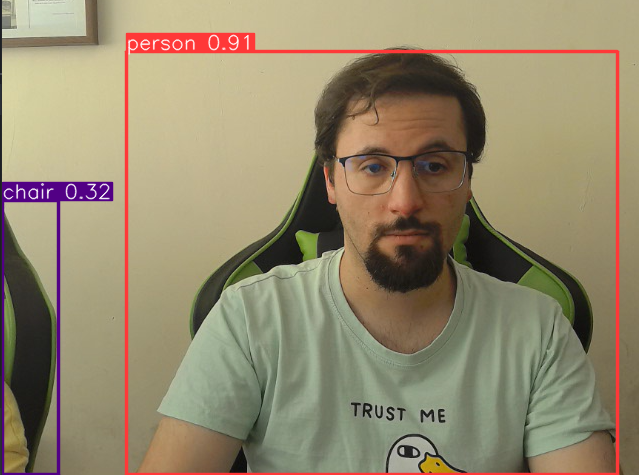
\includegraphics{imgs/camara sin tracker.png}
\caption{image}
\end{figure}

    \subsection{Con Track}\label{con-track}

    \begin{tcolorbox}[breakable, size=fbox, boxrule=1pt, pad at break*=1mm,colback=white, colframe=black]
\prompt{In}{incolor}{2}{\boxspacing}
\begin{Verbatim}[commandchars=\\\{\}]
\PY{k+kn}{from} \PY{n+nn}{ultralytics} \PY{k+kn}{import} \PY{n}{YOLO}
\PY{c+c1}{\PYZsh{} Instancia del modelo YOLO con los pesos especificados}
\PY{n}{pesos\PYZus{}yolo} \PY{o}{=} \PY{l+s+s2}{\PYZdq{}}\PY{l+s+s2}{yolov8n.pt}\PY{l+s+s2}{\PYZdq{}}
\PY{n}{model} \PY{o}{=} \PY{n}{YOLO}\PY{p}{(}\PY{n}{pesos\PYZus{}yolo}\PY{p}{)}
\PY{k}{try}\PY{p}{:}
\PY{c+c1}{\PYZsh{} Realiza la detección de objetos en el flujo de video de la cámara del computador}
 \PY{n}{results} \PY{o}{=} \PY{n}{model}\PY{o}{.}\PY{n}{track}\PY{p}{(}\PY{n}{source}\PY{o}{=}\PY{l+m+mi}{1}\PY{p}{,} \PY{n}{show}\PY{o}{=}\PY{k+kc}{True}\PY{p}{,} \PY{n}{conf}\PY{o}{=}\PY{l+m+mf}{0.3}\PY{p}{,} \PY{n}{save}\PY{o}{=}\PY{k+kc}{True}\PY{p}{)}
\PY{k}{except} \PY{n+ne}{Exception} \PY{k}{as} \PY{n}{e}\PY{p}{:}
    \PY{n+nb}{print}\PY{p}{(}\PY{l+s+s2}{\PYZdq{}}\PY{l+s+s2}{Ocurrió un error al realizar la detección de objetos:}\PY{l+s+s2}{\PYZdq{}}\PY{p}{,} \PY{n}{e}\PY{p}{)} 
\end{Verbatim}
\end{tcolorbox}

\begin{tcolorbox}[breakable, size=fbox, boxrule=1pt, pad at break*=1mm,colback=cellbackground, colframe=cellborder]
    \prompt{Out}{outcolor}{2}{\boxspacing}
    \begin{Verbatim}[commandchars=\\\{\}]

1/1: 1{\ldots} Success  (inf frames of shape 640x480 at 30.00 FPS)


WARNING  inference results will accumulate in RAM unless `stream=True` is
passed, causing potential out-of-memory
errors for large sources or long-running streams and videos. See
https://docs.ultralytics.com/modes/predict/ for help.

Example:
    results = model(source={\ldots}, stream=True)  \# generator of Results objects
    for r in results:
        boxes = r.boxes  \# Boxes object for bbox outputs
        masks = r.masks  \# Masks object for segment masks outputs
        probs = r.probs  \# Class probabilities for classification outputs

0: 480x640 1 person, 95.0ms
0: 480x640 1 person, 78.0ms
0: 480x640 1 person, 77.1ms
0: 480x640 1 person, 76.0ms
0: 480x640 1 person, 80.0ms
0: 480x640 1 person, 76.0ms
    \end{Verbatim}
\end{tcolorbox}

    \begin{figure}
\centering
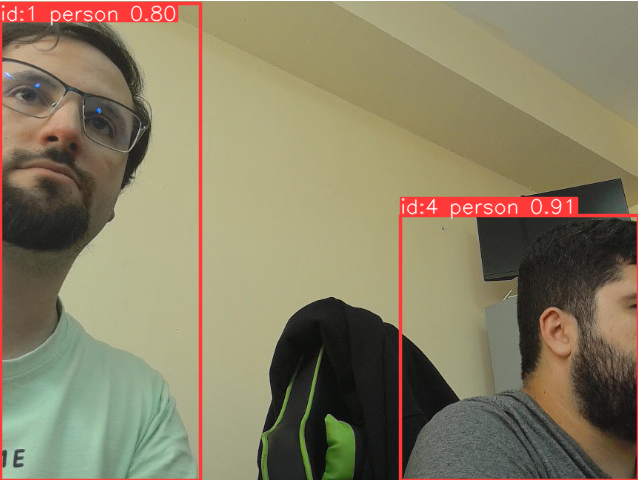
\includegraphics{imgs/camara con tracker.png}
\caption{image}
\end{figure}

    \section{Entrenamiento en Google
Colab}\label{entrenamiento-en-google-colab}

    Para usar la GPU, es mejor usar
\href{https://colab.research.google.com/drive/1kdhELxiiiV_b1F85cdr8fet8iHr_7gVU?usp=sharing}{Google
colab}. Para ello vamos a seguir los siguientes pasos:

    \subsection{Configurar Google
Colab}\label{configurar-google-colab}

    En Google Colab, seleccionamos la opción ``Entorno de ejecución'' y
luego ``Cambiar tipo de entorno de ejecución''.

    \begin{figure}
\centering
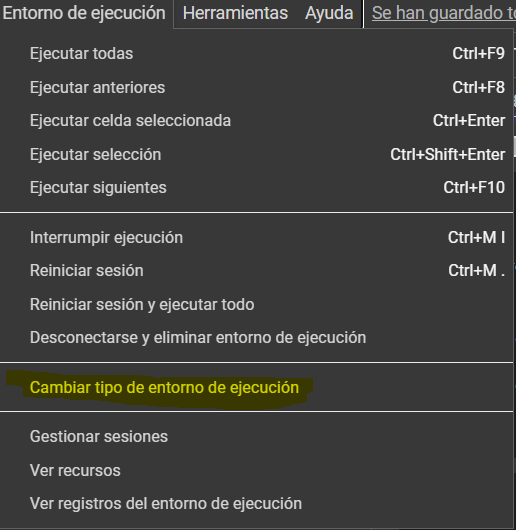
\includegraphics{imgs/Cambiar entorno a GPU.png}
\caption{image}
\end{figure}

    Ahora, marcamos la opción ``T4 GPU''.

    \begin{figure}
\centering
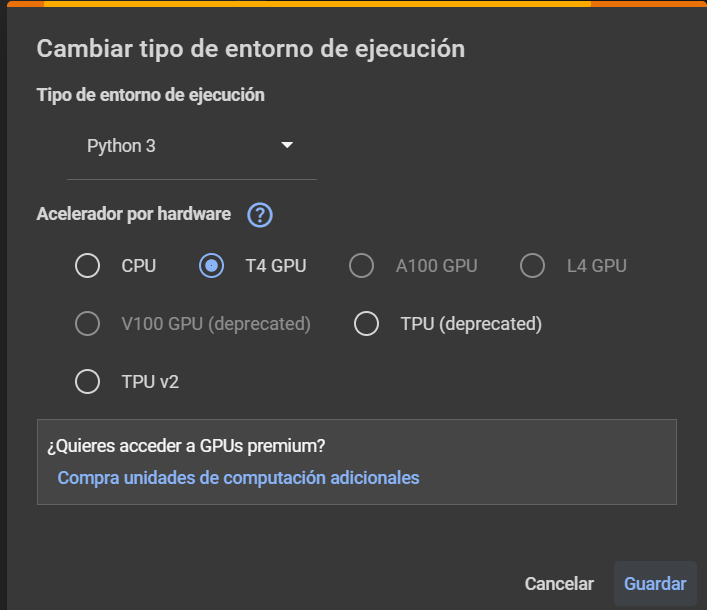
\includegraphics[width=0.7\textwidth]{imgs/Seleccionar T4 GPU.png}
\caption{image}
\end{figure}

    Y listo, con esto ya estaria configurado Google Colab para usar GPU en
vez de CPU. Lo podemos comprobar con el siguiente codigo.

    \begin{figure}
\centering
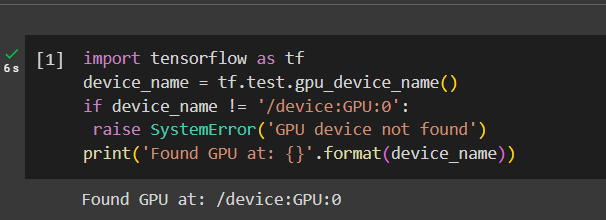
\includegraphics{imgs/Comprobamos que usa la GPU.png}
\caption{image}
\end{figure}

    Ahora, comprobamos la diferencia de usar GPU vs usar CPU.

    \begin{figure}
\centering
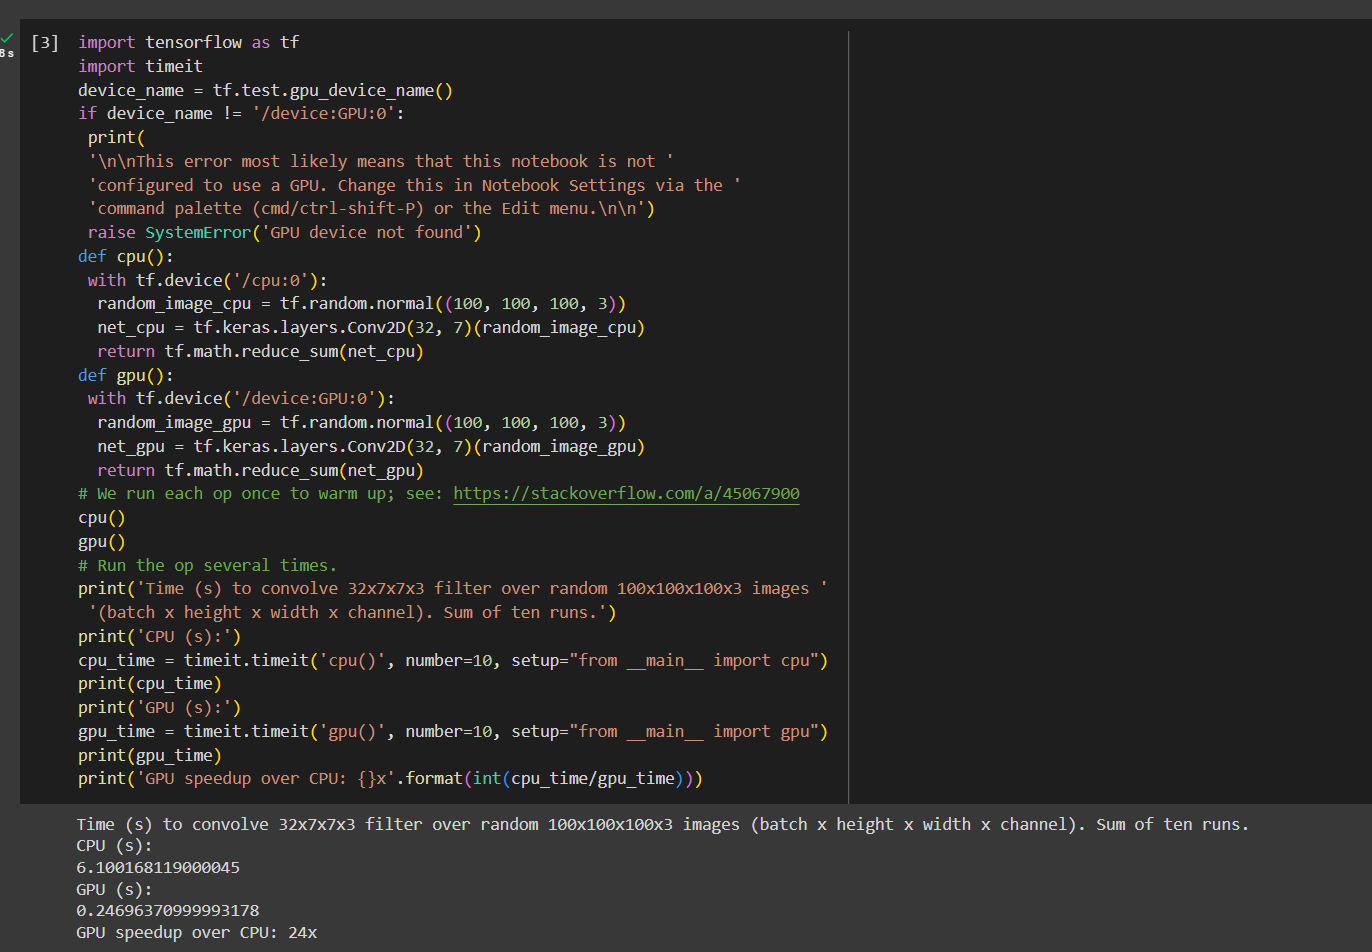
\includegraphics{imgs/Comprobamos que lee las imagenes mas rapido.png}
\caption{images}
\end{figure}

    Como podemos comprobar, la GPU carga la imagen 6 veces mas rapido que la
CPU.

    \subsection{Instalar dependencia}\label{instalar-dependencia}

    Para poder entrenar nuestro modelo lo primero que necesitamos es
instalar ultralystics en el entorno de Google Colab

    \begin{figure}
\centering
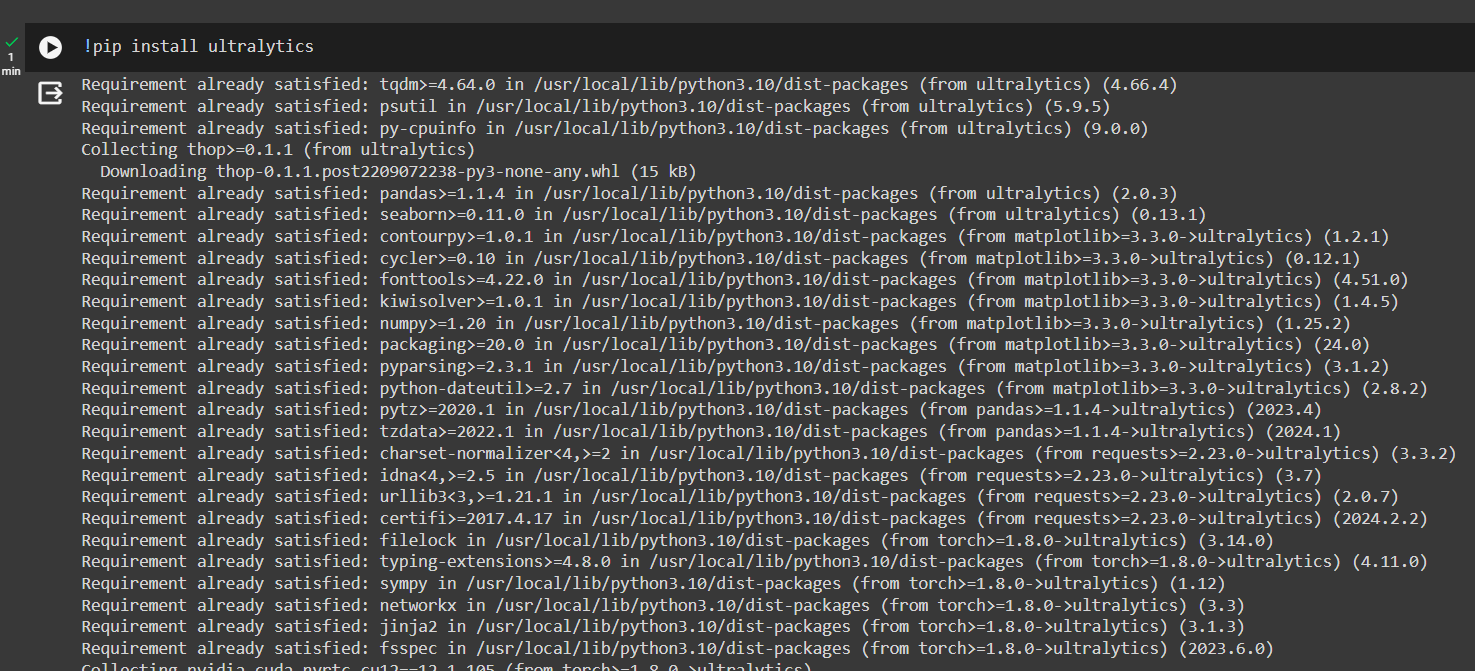
\includegraphics{imgs/Instalamos Ultralystics.png}
\caption{imagen}
\end{figure}

    \subsection{Cargar modelo}\label{cargar-modelo}

    Una vez instalado ya podemos cargar el modelo de YOLO con los pesos
pre-entrenados

    \begin{figure}
\centering
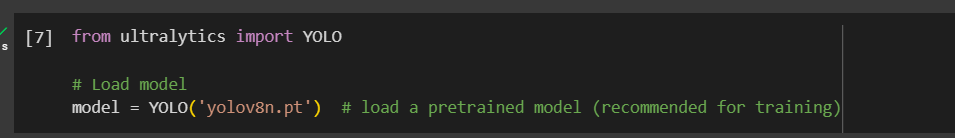
\includegraphics{imgs/Cargamos el modelo.png}
\caption{images}
\end{figure}

    \subsection{Subir y descomprimir
Dataset}\label{subir-y-descomprimir-dataset}

    Subimos el dataset en un archivo comprimido (Zip) y lo descomprimir con
el siguiente codigo.

    \begin{figure}
\centering
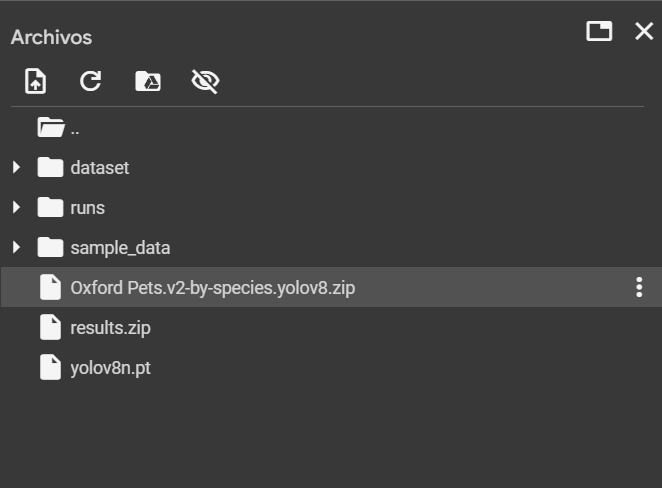
\includegraphics[width=0.7\textwidth]{imgs/Subimos el dataset para entrenar el modelo.png}
\caption{image}
\end{figure}

    \begin{figure}
\centering
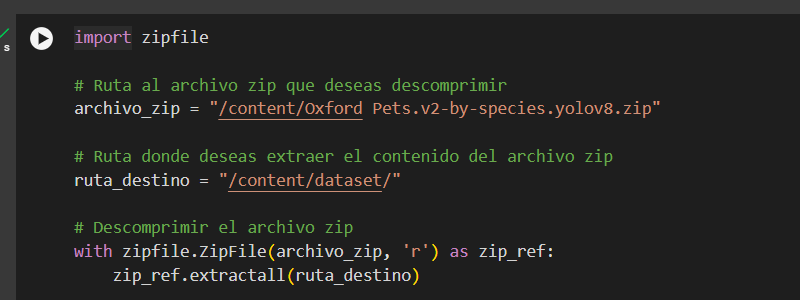
\includegraphics{imgs/Lo descomprimimos .png}
\caption{image}
\end{figure}

    \begin{figure}
\centering
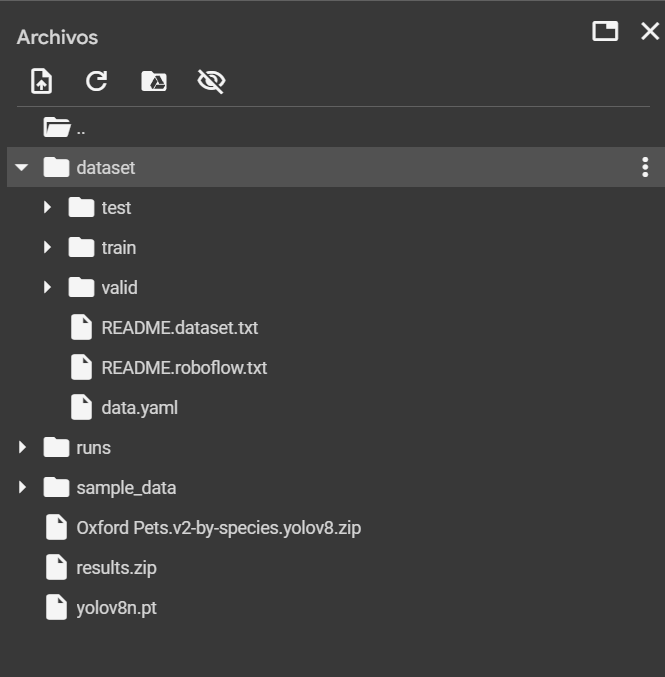
\includegraphics{imgs/Comprobamos que se descomprimio bien.png}
\caption{image}
\end{figure}

    \subsection{Entrenamiento del
modelo}\label{entrenamiento-del-modelo}

    \begin{figure}
\centering
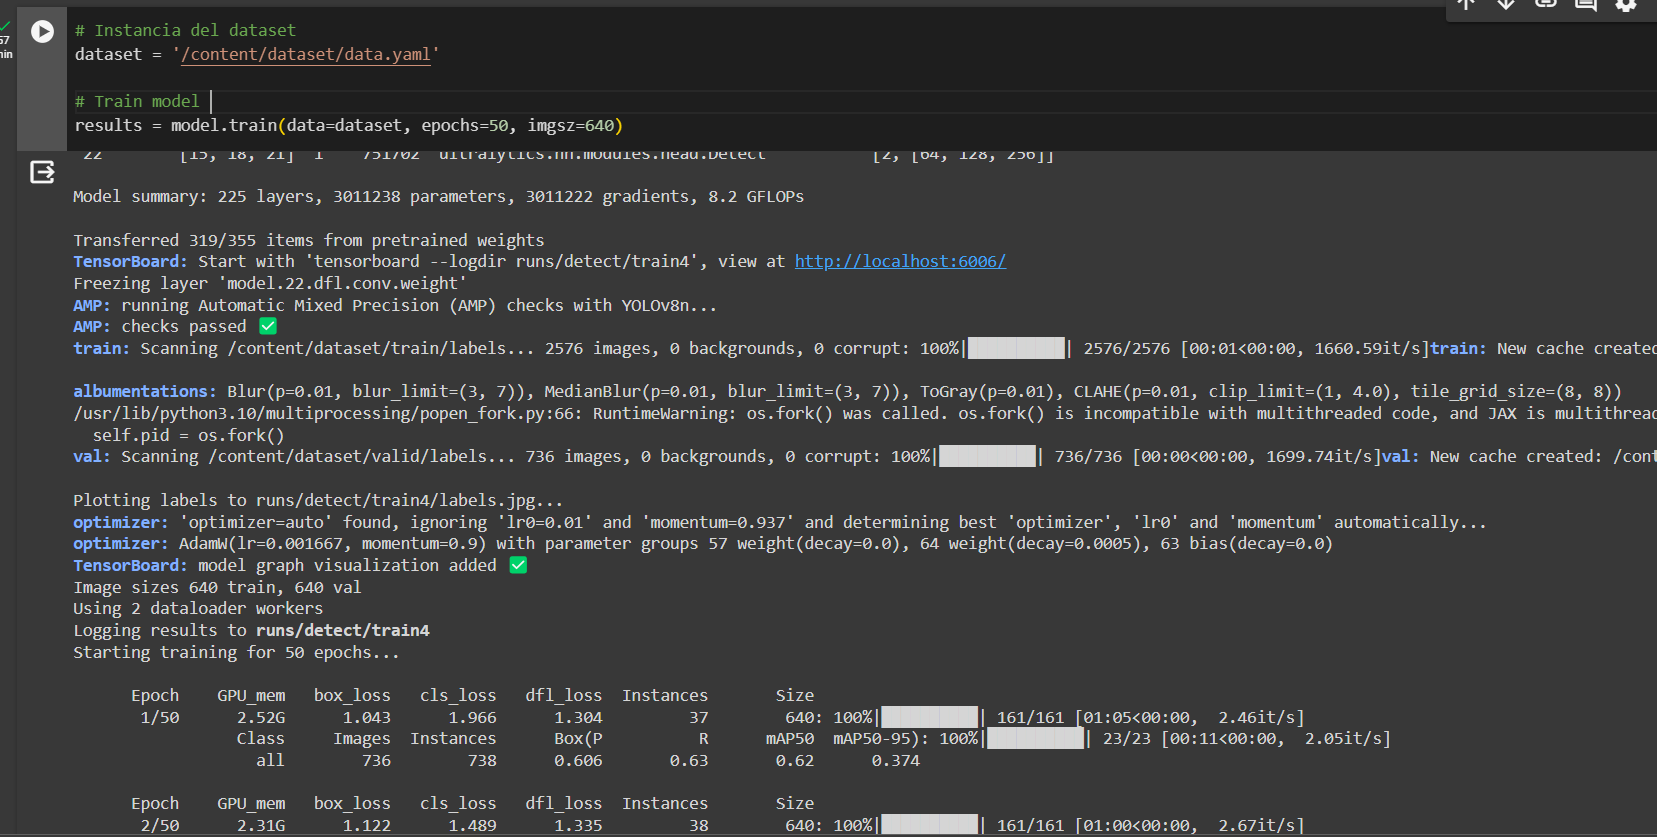
\includegraphics{imgs/Entrenamos el modelo.png}
\caption{images}
\end{figure}

    \subsection{Comprimir y descargar los
resultados}\label{comprimir-y-descargar-los-resultados}

    Una vez terminado el entrenamiento se generará una carpeta donde esta
guardado todos los pesos del modelo con las graficas pertinentes.

    \begin{figure}
\centering
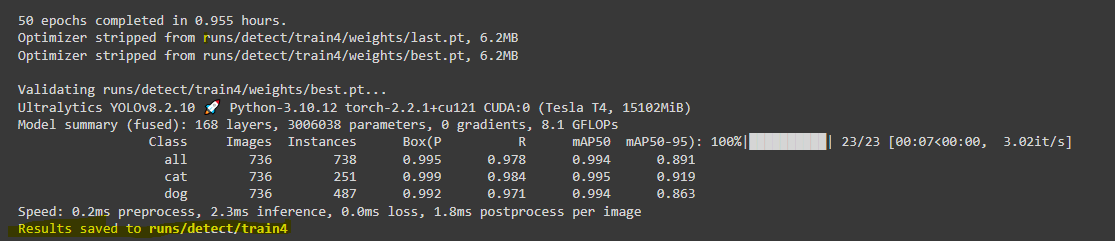
\includegraphics{imgs/Resultados.png}
\caption{images}
\end{figure}

    Ahora comprimimos la carpeta generada y la descargamos

    \begin{figure}
\centering
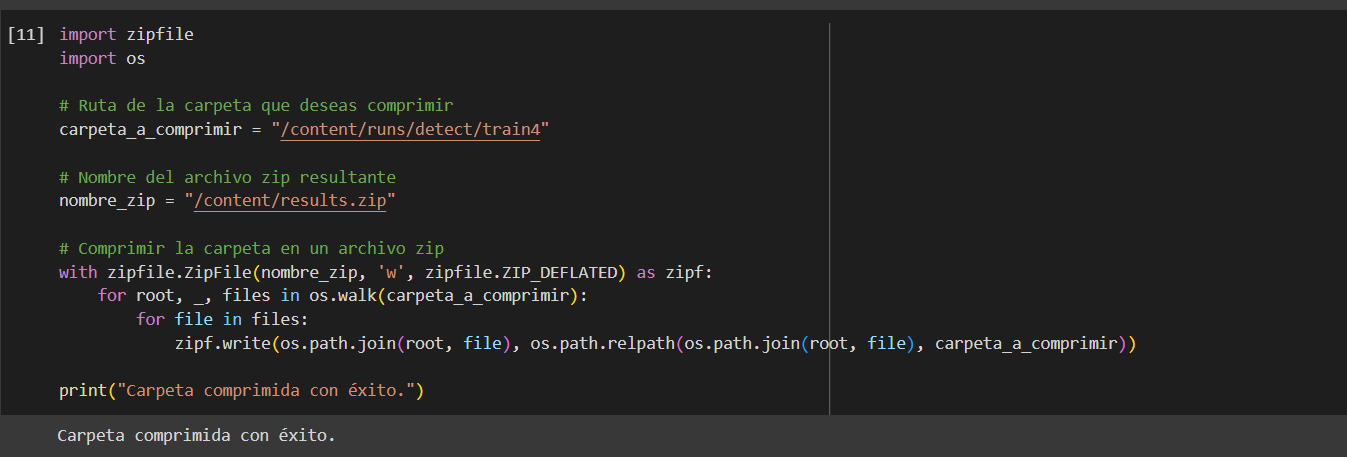
\includegraphics{imgs/Comprimimos los resultados para descargar.png}
\caption{images}
\end{figure}

    \section{Resultados del
entrenamiento}\label{resultados-del-entrenamiento}

    \begin{figure}
\centering
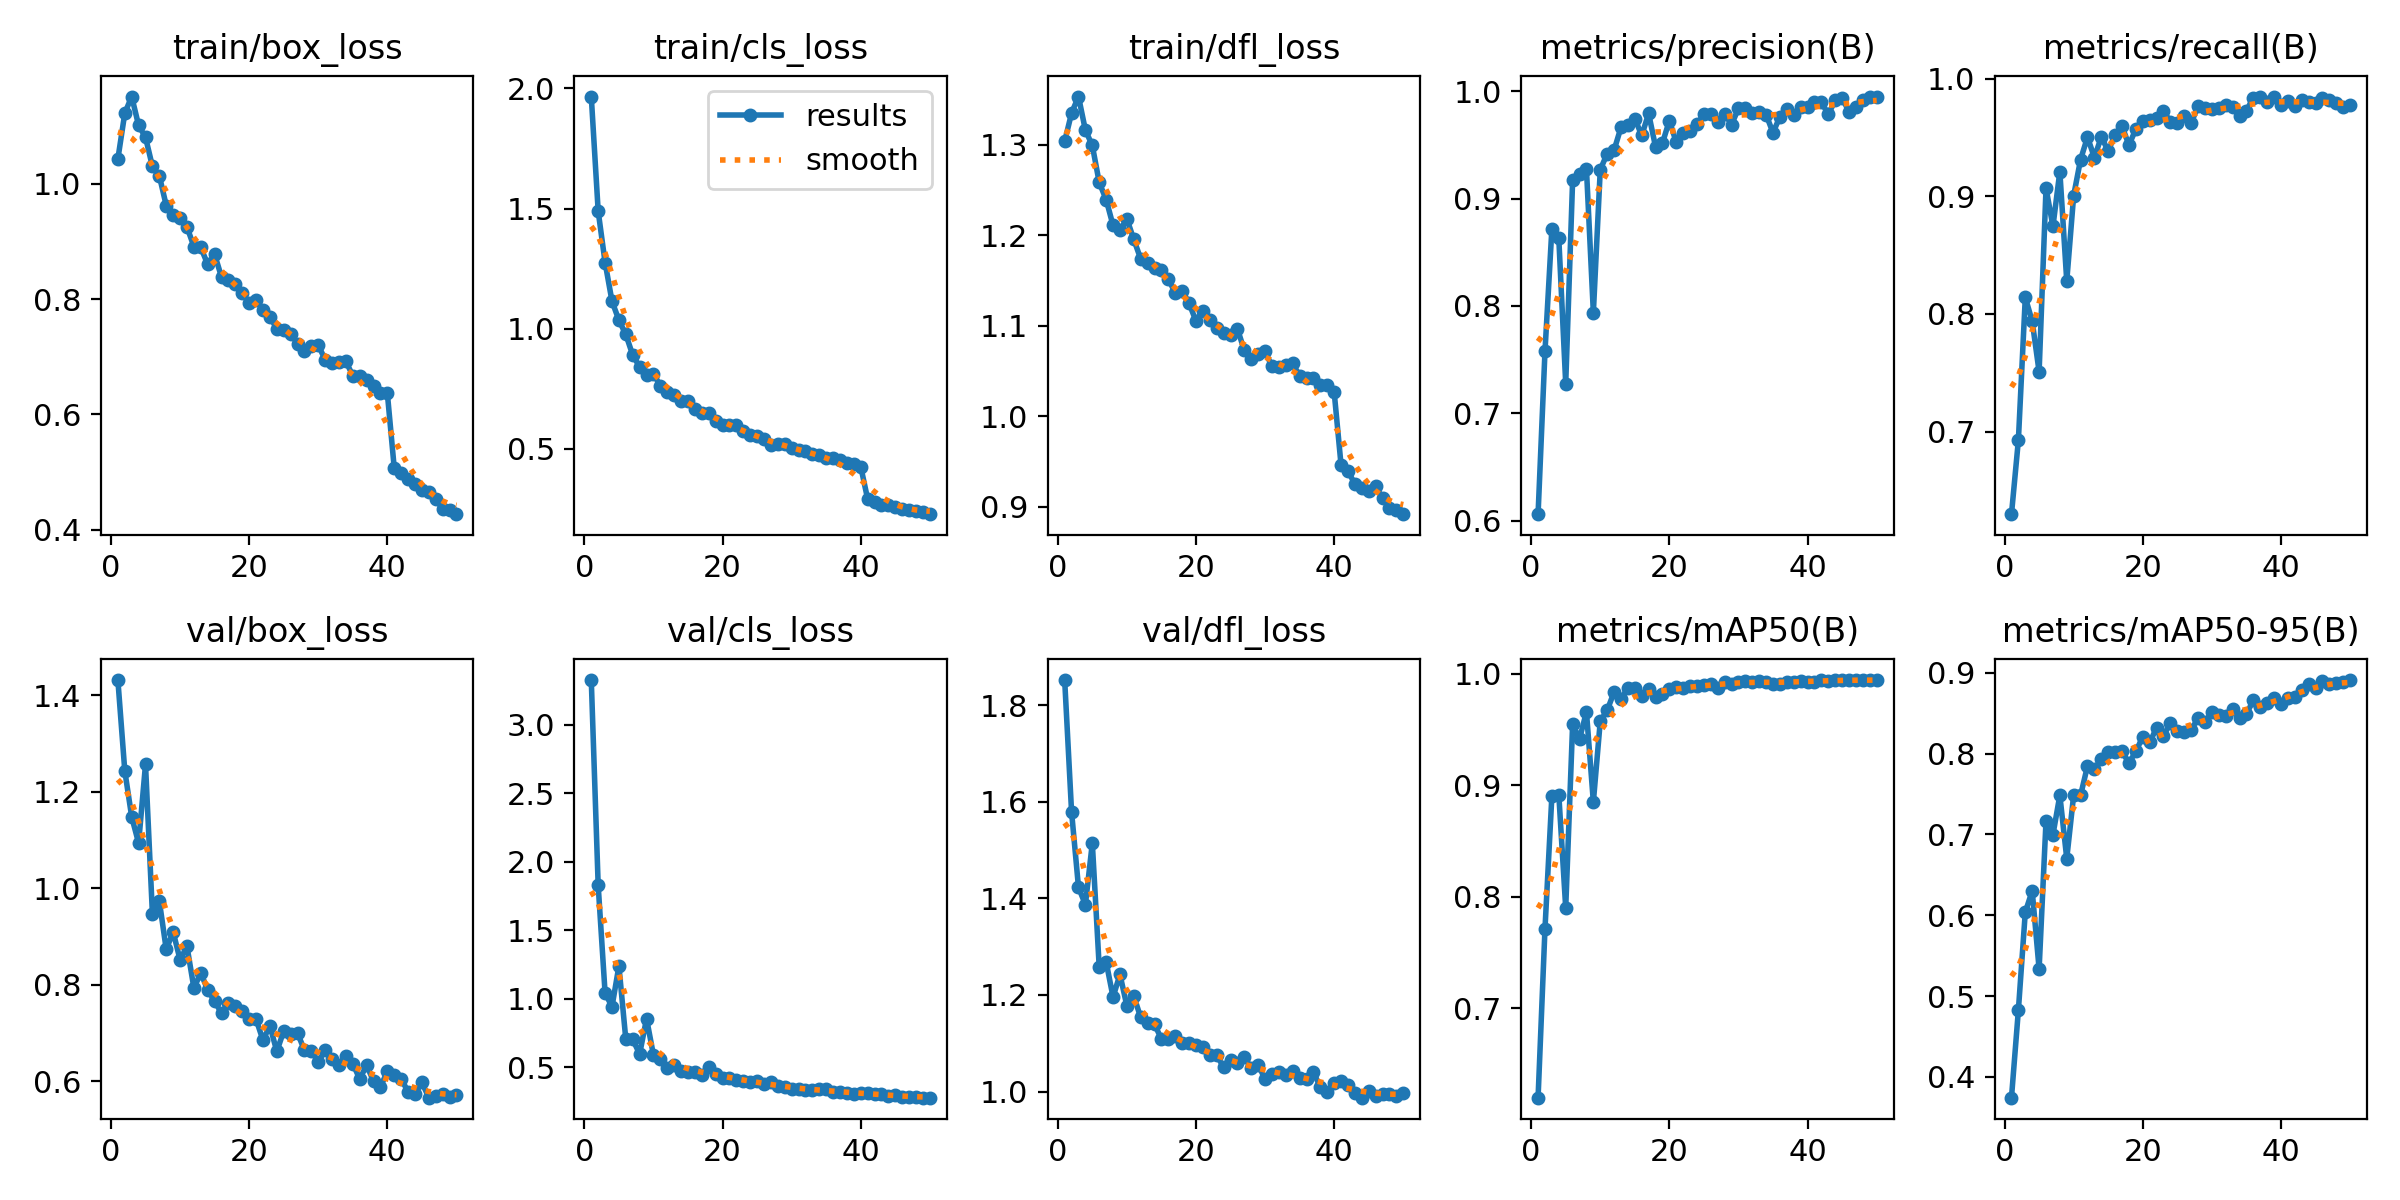
\includegraphics{results/results.png}
\caption{images}
\end{figure}

    \subsection{Matriz de confusión}\label{matriz-de-confusiuxf3n}

    \begin{figure}
\centering
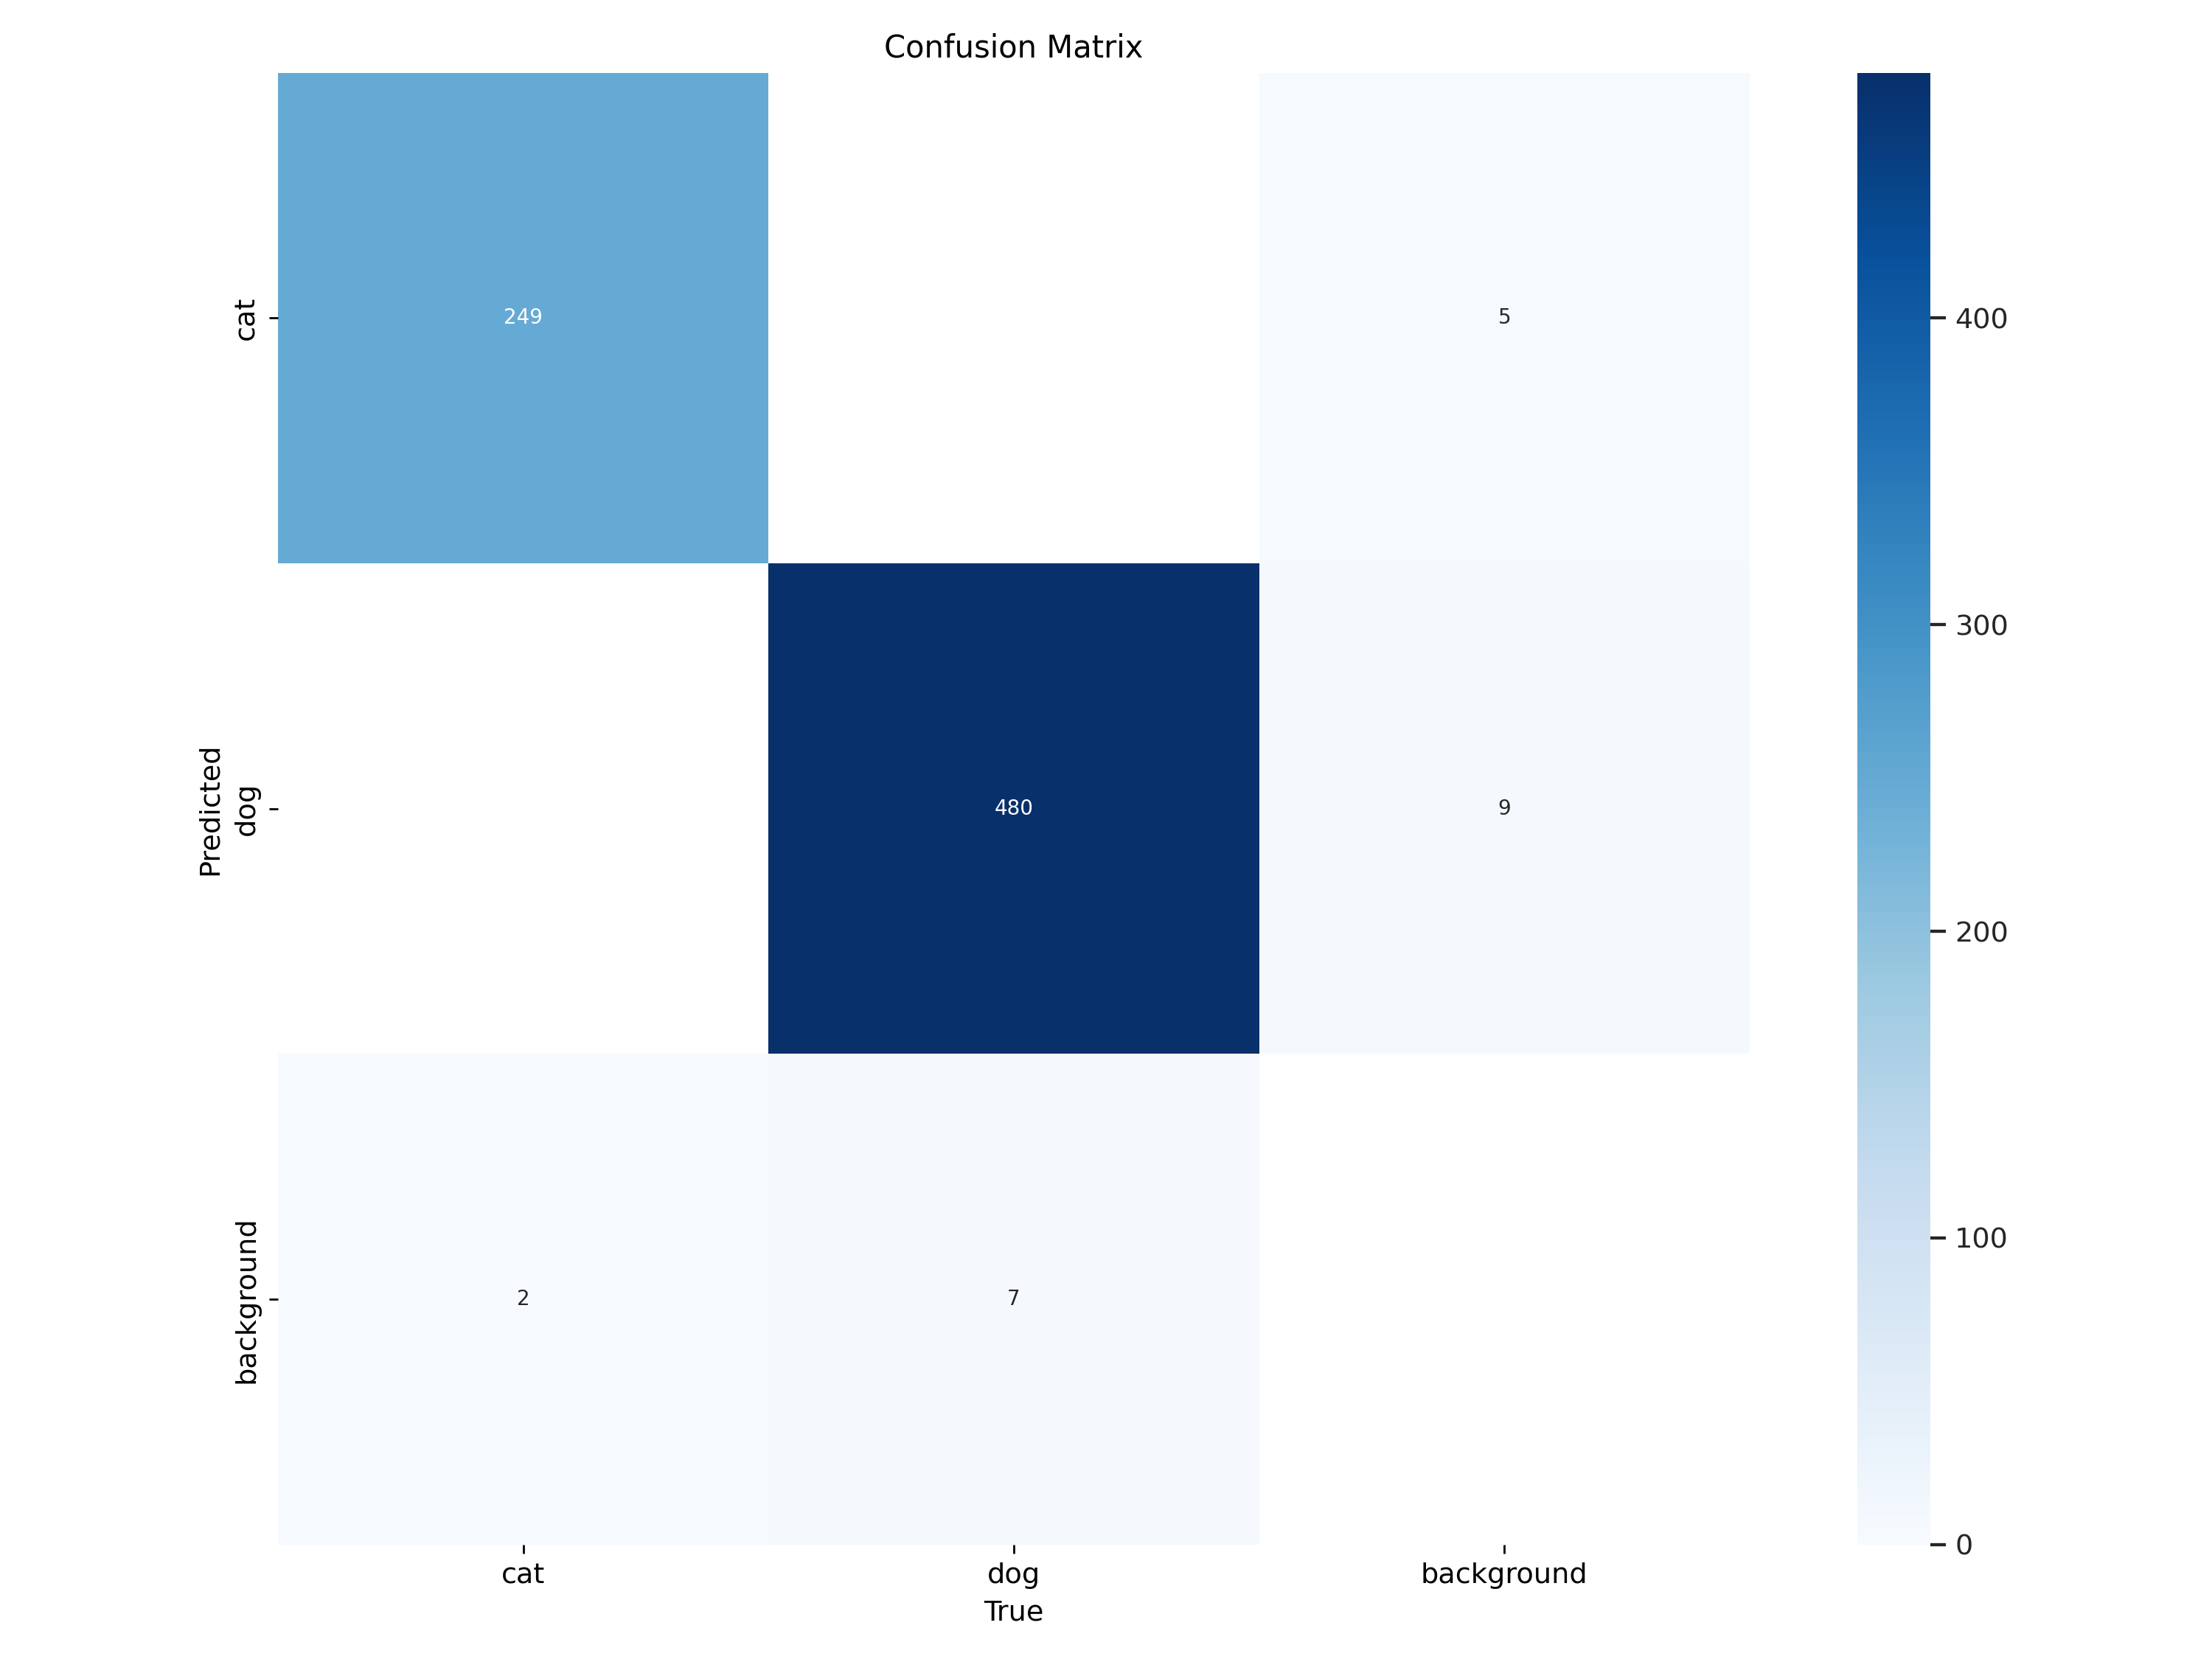
\includegraphics{results/confusion_matrix.png}
\caption{images}
\end{figure}

\subsection{Curva de Recall}\label{curva-de-recall}

    \begin{figure}
\centering
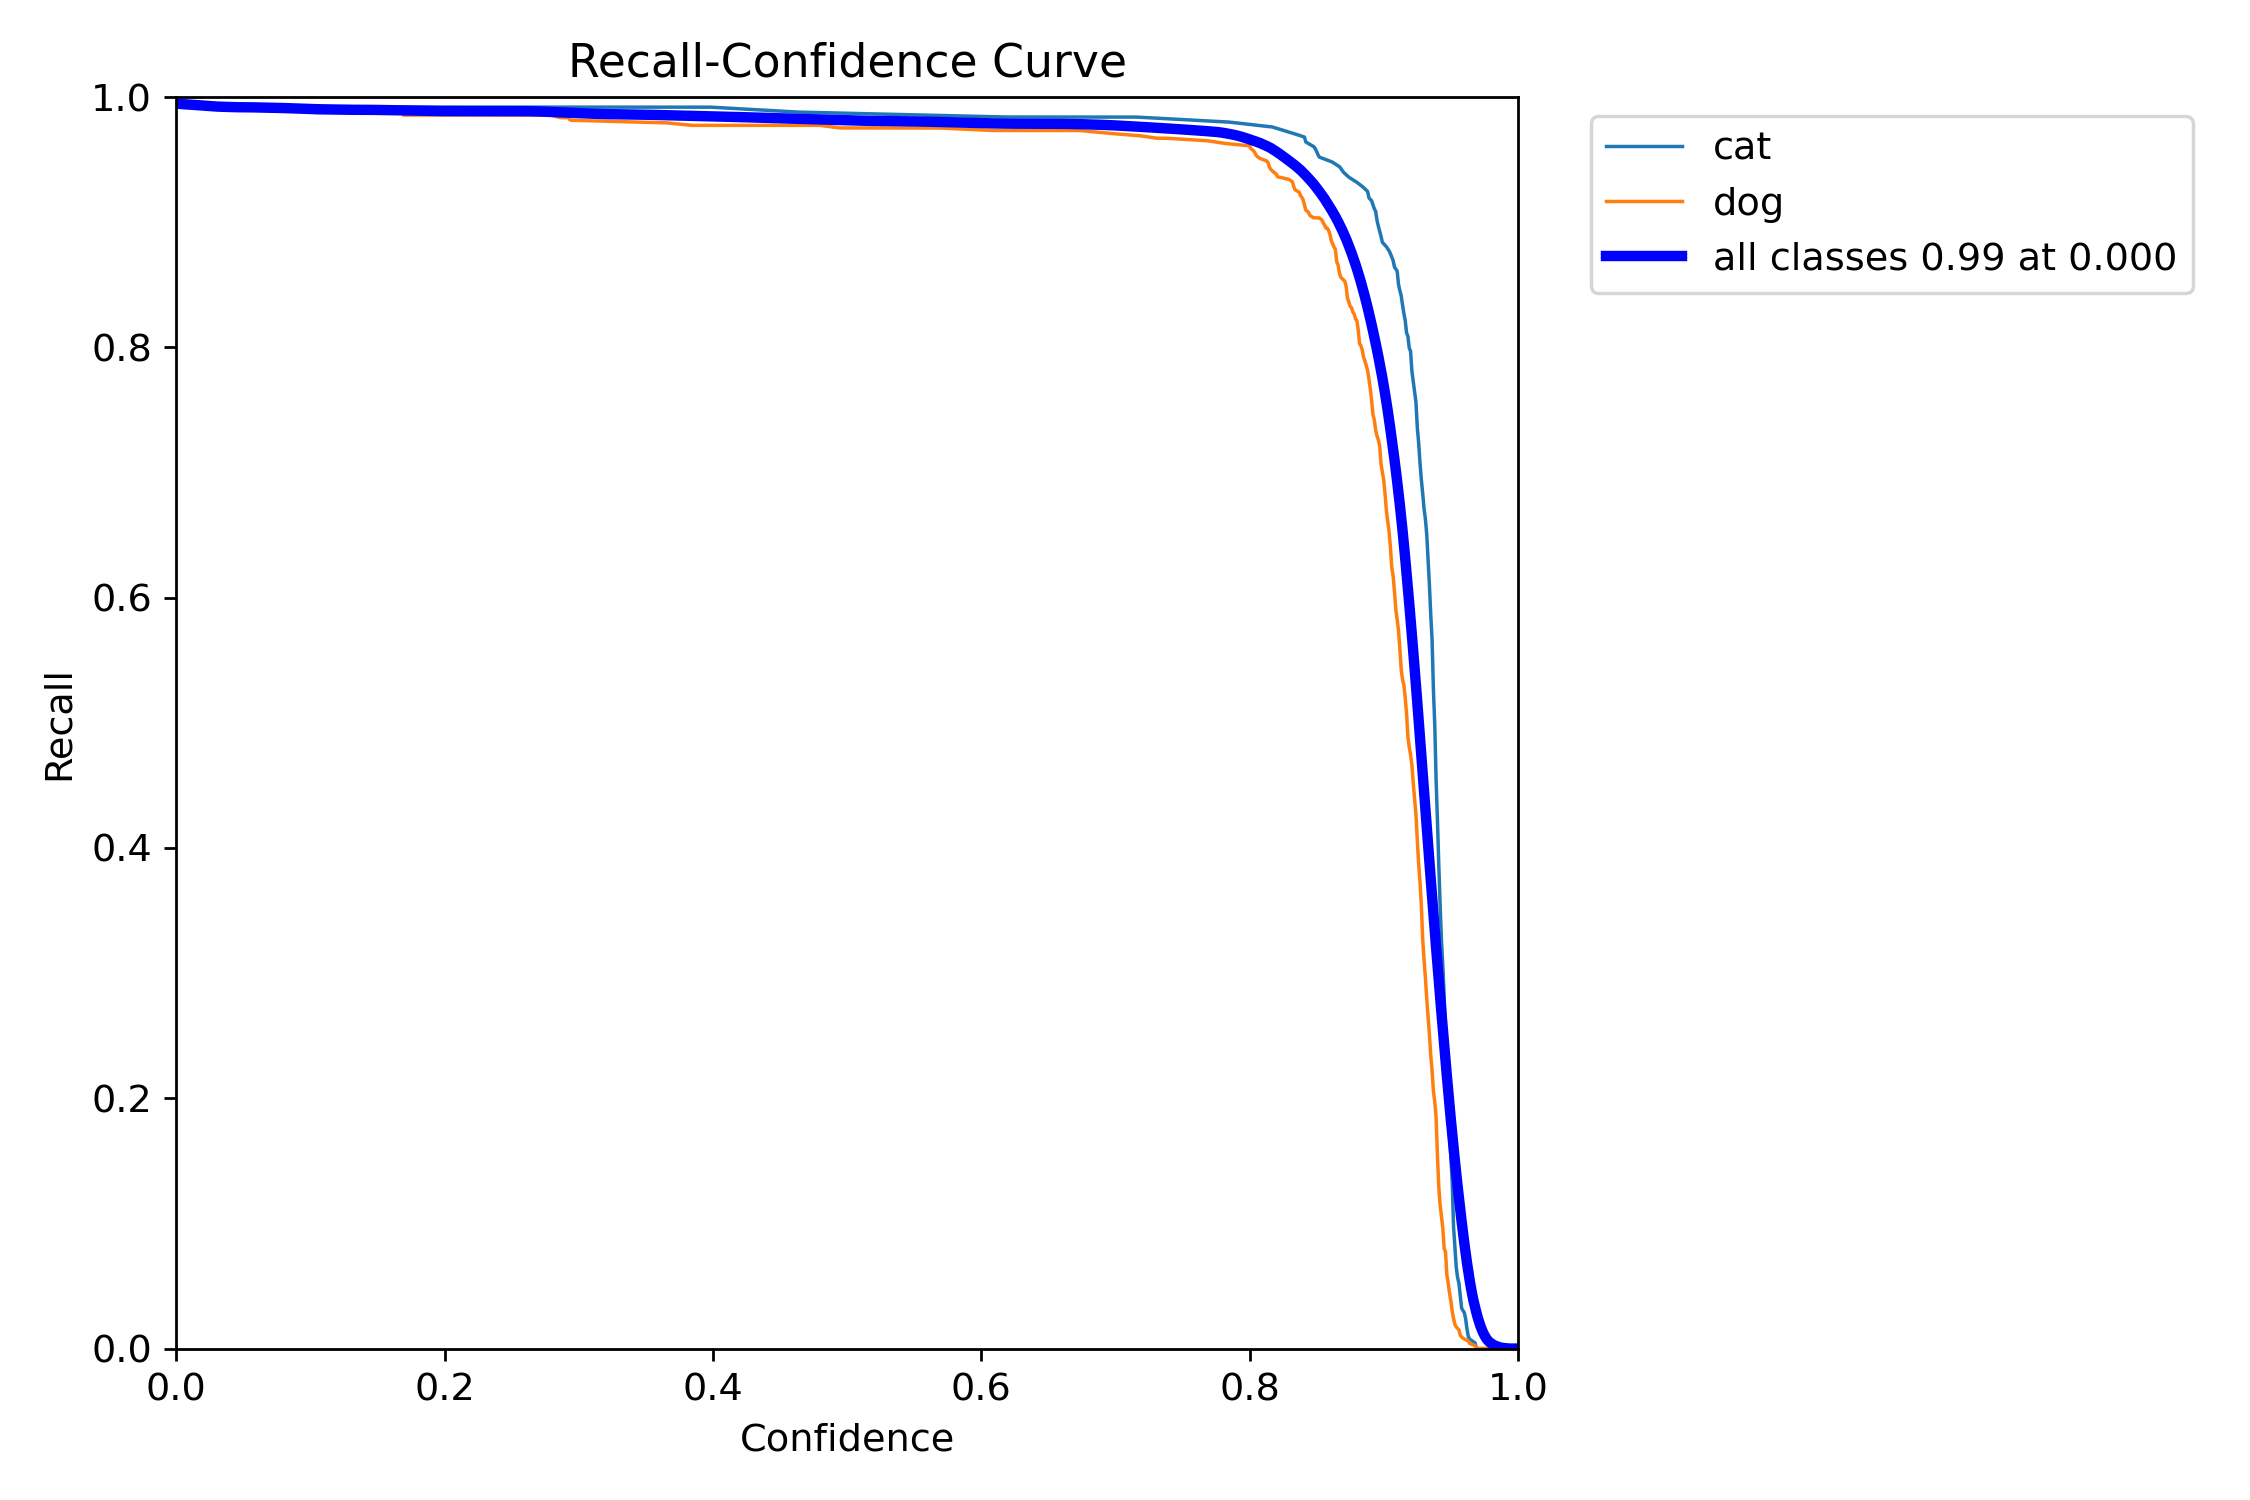
\includegraphics{results/R_curve.png}
\caption{images}
\end{figure}

    \subsection{Predicción con imagenes de
val}\label{predicciuxf3n-con-imagenes-de-val}

    \begin{figure}
\centering
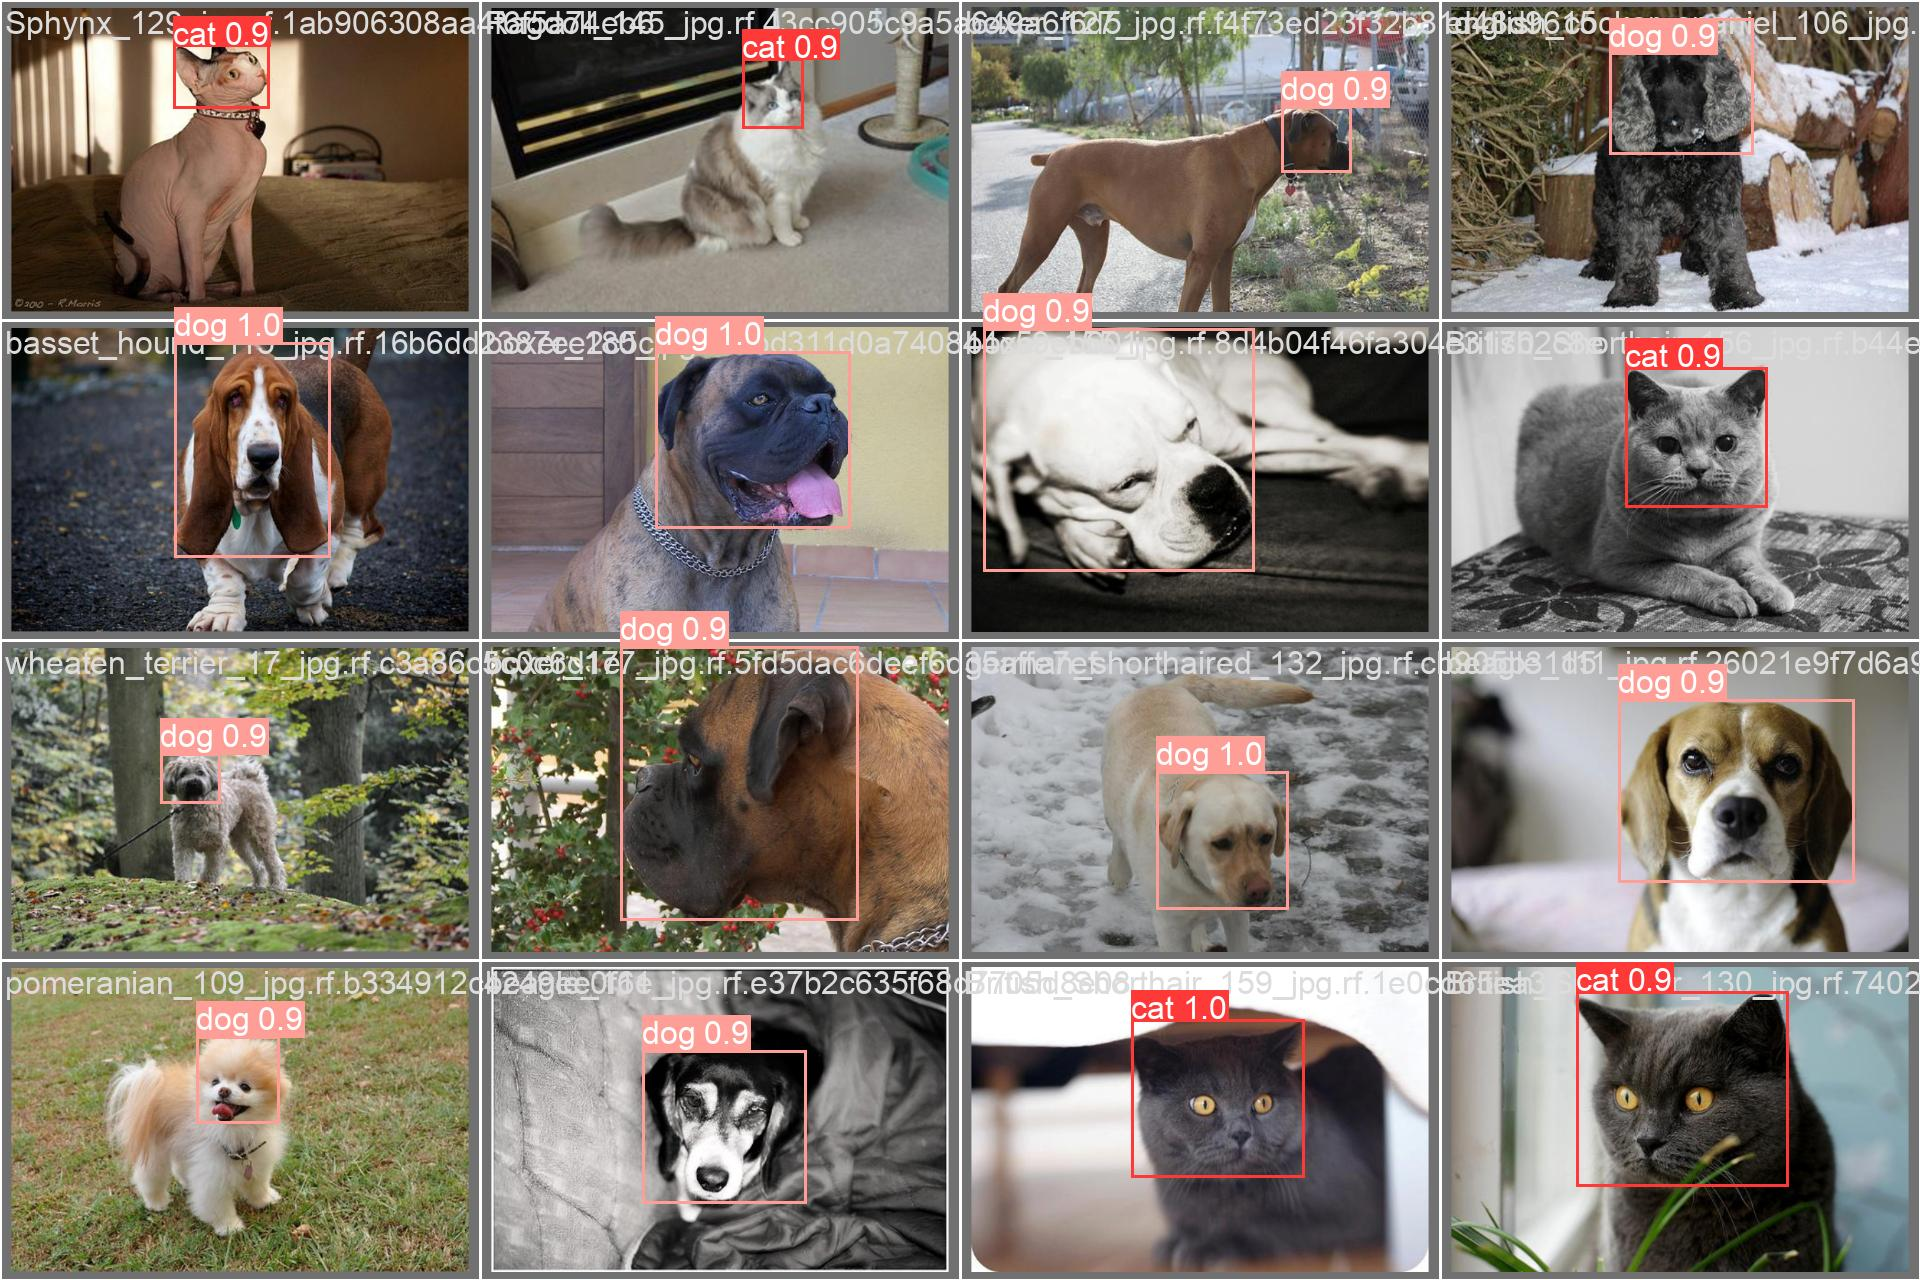
\includegraphics{results/val_batch1_pred.jpg}
\caption{images}
\end{figure}

    \section{Predicciones}\label{predicciones}

    \subsection{Predicciones con
imagenes}\label{predicciones-con-imagenes}

    \paragraph{Imagenes a predecir}\label{imagenes-a-predecir}

    \begin{longtable}[]{@{}
  >{\centering\arraybackslash}p{(\columnwidth - 4\tabcolsep) * \real{0.3333}}
  >{\centering\arraybackslash}p{(\columnwidth - 4\tabcolsep) * \real{0.3333}}
  >{\centering\arraybackslash}p{(\columnwidth - 4\tabcolsep) * \real{0.3333}}@{}}
\toprule\noalign{}
\begin{minipage}[b]{\linewidth}\centering
Imagen 1
\end{minipage} & \begin{minipage}[b]{\linewidth}\centering
Imagen 2
\end{minipage} & \begin{minipage}[b]{\linewidth}\centering
Imagen 3
\end{minipage} \\
\midrule\noalign{}
\endhead
\bottomrule\noalign{}
\endlastfoot
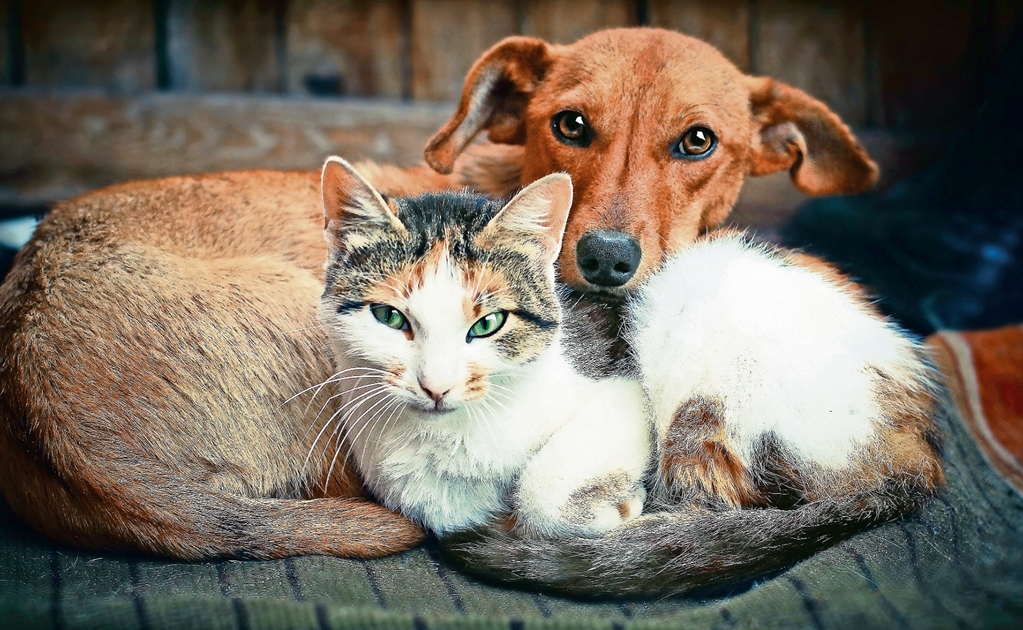
\includegraphics{test_img/cat and dog 1.jpg} &
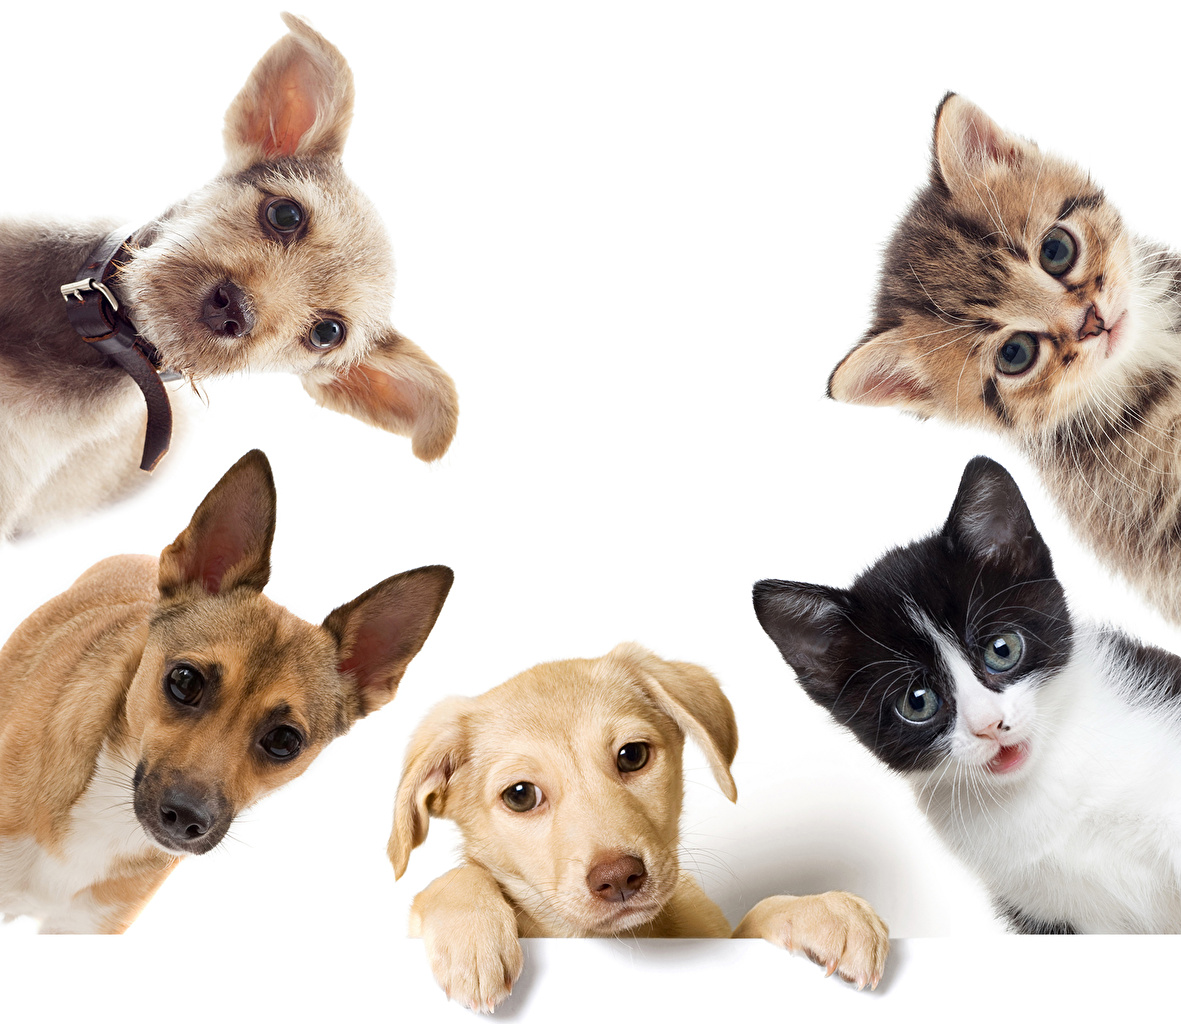
\includegraphics{test_img/cats and dogs.jpg} &
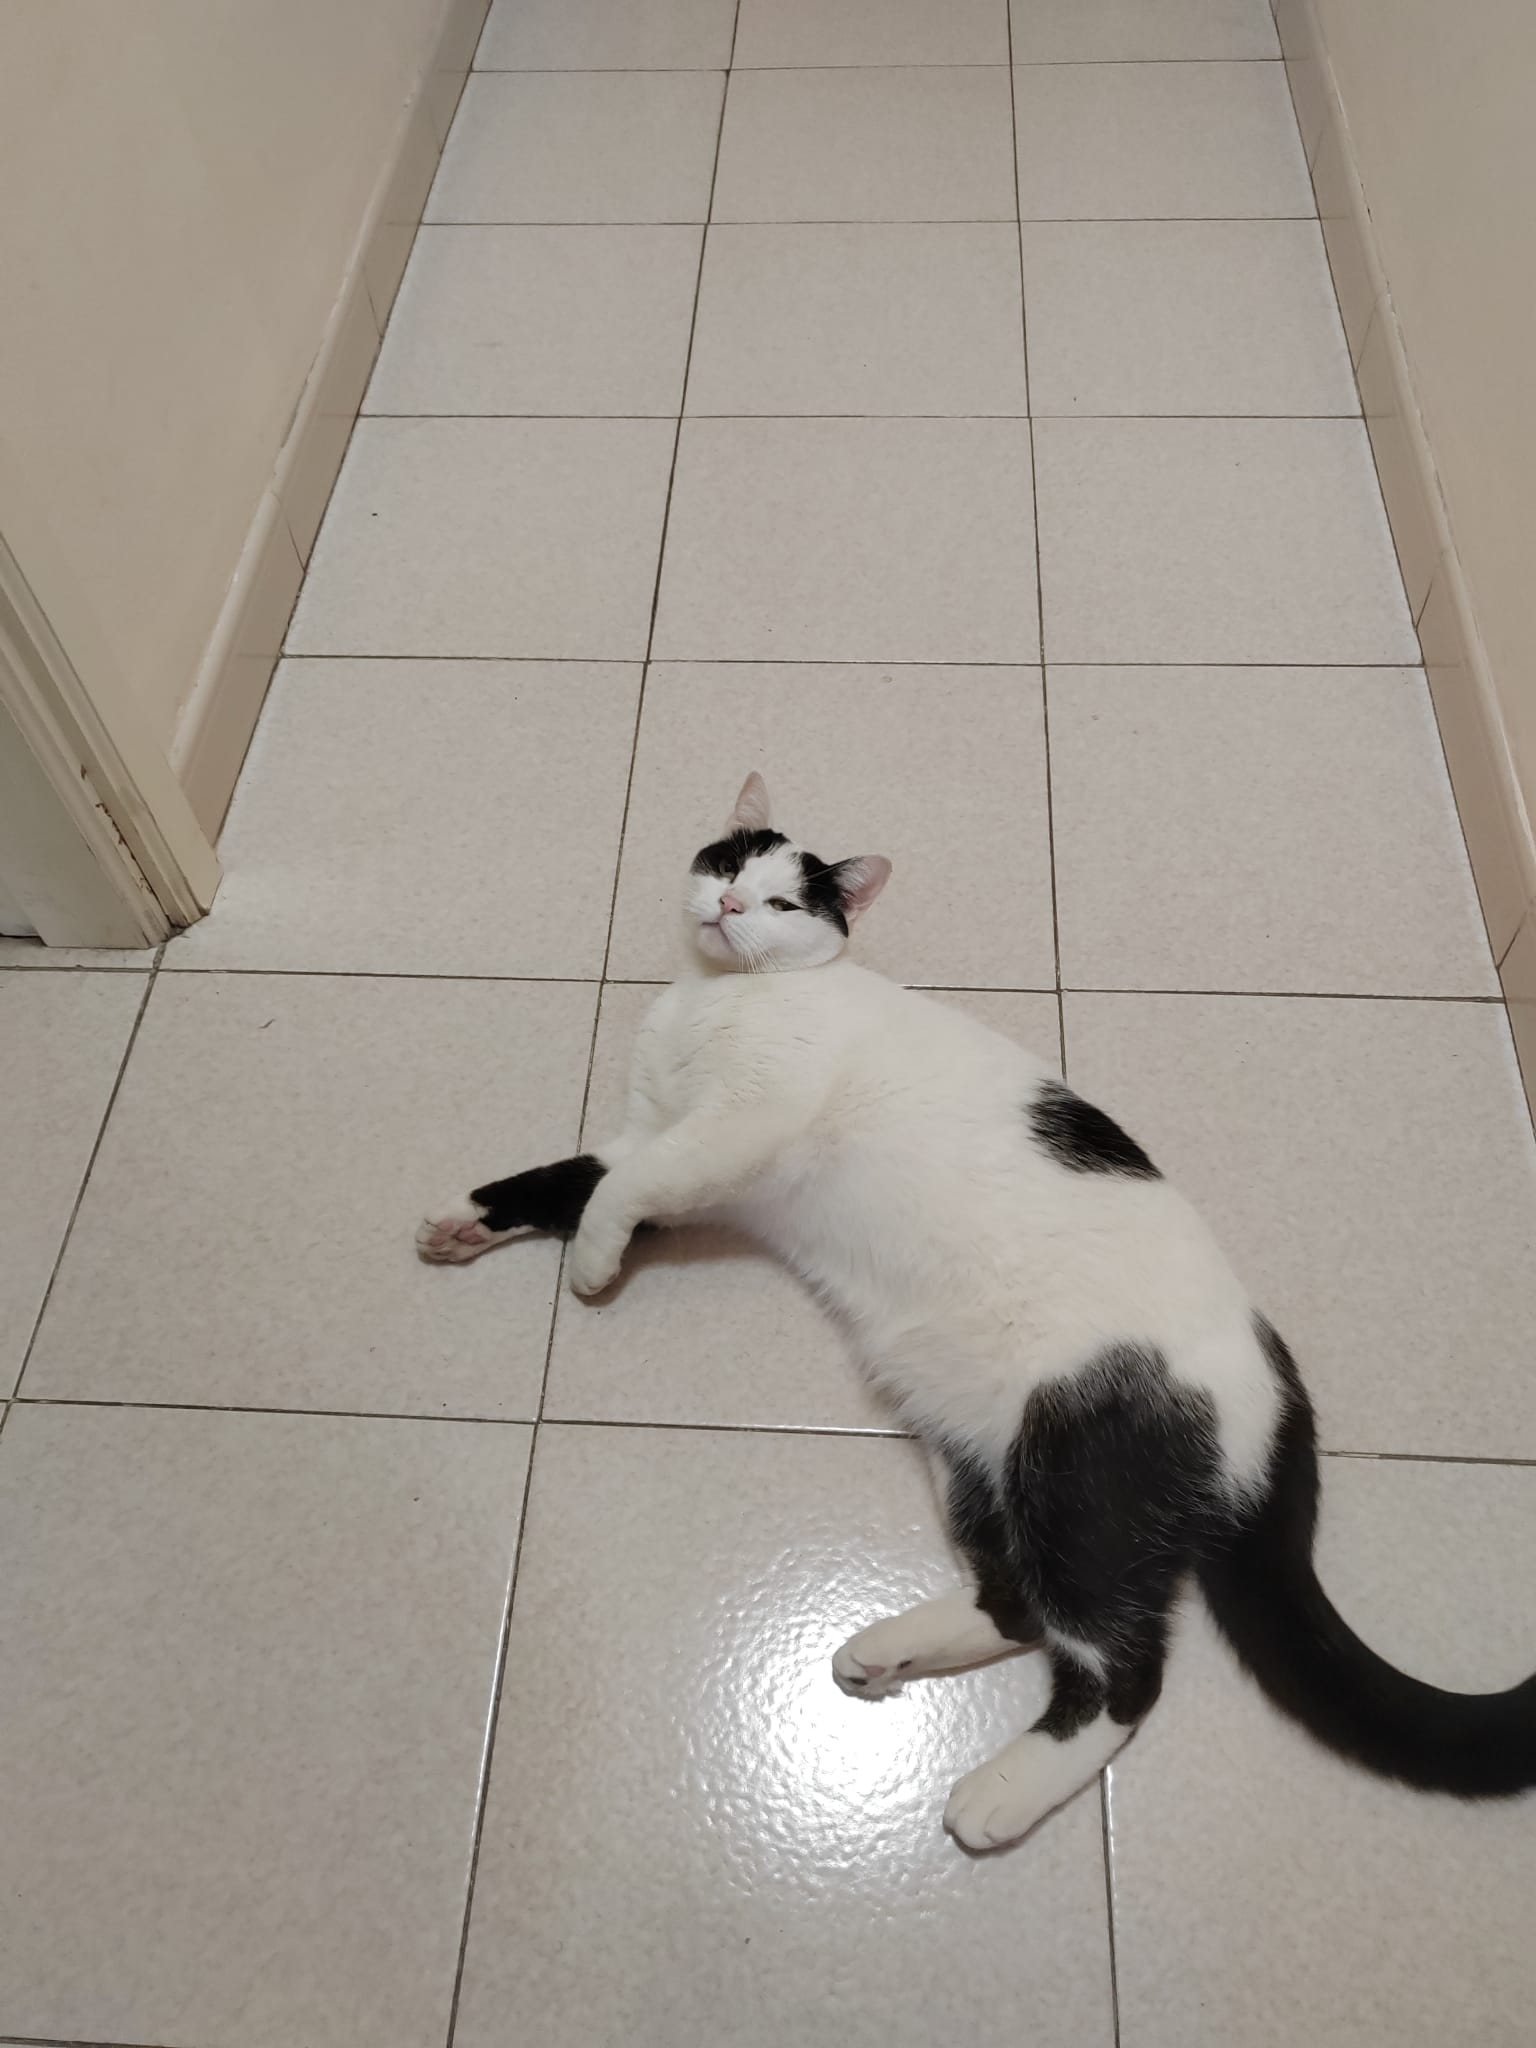
\includegraphics{test_img/cat.jpg} \\
\end{longtable}

    \paragraph{Predicción}\label{predicciuxf3n}
    { \hspace*{\fill} \\}

    \begin{tcolorbox}[breakable, size=fbox, boxrule=1pt, pad at break*=1mm,colback=white, colframe=black]
\prompt{In}{incolor}{3}{\boxspacing}
\begin{Verbatim}[commandchars=\\\{\}]
\PY{k+kn}{from} \PY{n+nn}{ultralytics} \PY{k+kn}{import} \PY{n}{YOLO}

\PY{n}{image\PYZus{}paths} \PY{o}{=} \PY{p}{[}\PY{l+s+s2}{\PYZdq{}}\PY{l+s+s2}{test\PYZus{}img/cats and dogs.jpg}\PY{l+s+s2}{\PYZdq{}}\PY{p}{,} \PY{l+s+s2}{\PYZdq{}}\PY{l+s+s2}{test\PYZus{}img/cat and dog 1.jpg}\PY{l+s+s2}{\PYZdq{}}\PY{p}{,} \PY{l+s+s2}{\PYZdq{}}\PY{l+s+s2}{test\PYZus{}img/cat.jpg}\PY{l+s+s2}{\PYZdq{}}\PY{p}{]}
\PY{c+c1}{\PYZsh{} Cargar el modelo YOLO preentrenado}
\PY{n}{model} \PY{o}{=} \PY{n}{YOLO}\PY{p}{(}\PY{l+s+s2}{\PYZdq{}}\PY{l+s+s2}{results/weights/best.pt}\PY{l+s+s2}{\PYZdq{}}\PY{p}{)}
\PY{c+c1}{\PYZsh{} Realizar la predicción en una imagen}
\PY{n}{results} \PY{o}{=} \PY{n}{model}\PY{o}{.}\PY{n}{track}\PY{p}{(}\PY{n}{source}\PY{o}{=}\PY{n}{image\PYZus{}paths}\PY{p}{,} \PY{n}{conf}\PY{o}{=}\PY{l+m+mf}{0.3}\PY{p}{,}
\PY{n}{iou}\PY{o}{=}\PY{l+m+mf}{0.5}\PY{p}{)} 
\PY{n}{i} \PY{o}{=} \PY{l+m+mi}{0}
\PY{c+c1}{\PYZsh{} Process results list}
\PY{k}{for} \PY{n}{result} \PY{o+ow}{in} \PY{n}{results}\PY{p}{:}
    \PY{n}{i}\PY{o}{+}\PY{o}{=}\PY{l+m+mi}{1}
    \PY{n}{boxes} \PY{o}{=} \PY{n}{result}\PY{o}{.}\PY{n}{boxes}  \PY{c+c1}{\PYZsh{} Boxes object for bounding box outputs}
    \PY{n}{result}\PY{o}{.}\PY{n}{show}\PY{p}{(}\PY{p}{)}  \PY{c+c1}{\PYZsh{} display to screen}
    \PY{n}{result}\PY{o}{.}\PY{n}{save}\PY{p}{(}\PY{n}{filename}\PY{o}{=} \PY{l+s+sa}{f}\PY{l+s+s2}{\PYZdq{}}\PY{l+s+s2}{predicts/predict }\PY{l+s+si}{\PYZob{}}\PY{n}{i}\PY{l+s+si}{\PYZcb{}}\PY{l+s+s2}{.jpg}\PY{l+s+s2}{\PYZdq{}}\PY{p}{)}
    \PY{k}{for} \PY{n}{box} \PY{o+ow}{in} \PY{n}{boxes}\PY{p}{:}
        \PY{n+nb}{print}\PY{p}{(}\PY{l+s+s2}{\PYZdq{}}\PY{l+s+s2}{Box:}\PY{l+s+s2}{\PYZdq{}}\PY{p}{,} \PY{n}{box}\PY{p}{)} 
\end{Verbatim}
\end{tcolorbox}

\begin{tcolorbox}[breakable, size=fbox, boxrule=1pt, pad at break*=1mm,colback=cellbackground, colframe=cellborder]
    \prompt{Out}{outcolor}{3}{\boxspacing}
    \begin{Verbatim}[commandchars=\\\{\}]

0: 640x640 2 cats, 3 dogs, 105.9ms
1: 640x640 1 cat, 1 dog, 105.9ms
2: 640x640 1 cat, 105.9ms
Speed: 5.0ms preprocess, 105.9ms inference, 0.7ms postprocess per image at shape
(1, 3, 640, 640)
Box: ultralytics.engine.results.Boxes object with attributes:

cls: tensor([1.])
conf: tensor([0.9455])
data: tensor([[131.1942, 448.6709, 454.5172, 851.3074,   1.0000,   0.9455,
1.0000]])
id: tensor([1.])
is\_track: True
orig\_shape: (1024, 1181)
shape: torch.Size([1, 7])
xywh: tensor([[292.8557, 649.9891, 323.3230, 402.6365]])
xywhn: tensor([[0.2480, 0.6348, 0.2738, 0.3932]])
xyxy: tensor([[131.1942, 448.6709, 454.5172, 851.3074]])
xyxyn: tensor([[0.1111, 0.4382, 0.3849, 0.8314]])
Box: ultralytics.engine.results.Boxes object with attributes:

cls: tensor([0.])
conf: tensor([0.9338])
data: tensor([[7.5364e+02, 4.5368e+02, 1.0768e+03, 7.7989e+02, 2.0000e+00,
9.3380e-01, 0.0000e+00]])
id: tensor([2.])
is\_track: True
orig\_shape: (1024, 1181)
shape: torch.Size([1, 7])
xywh: tensor([[915.2371, 616.7838, 323.2015, 326.2104]])
xywhn: tensor([[0.7750, 0.6023, 0.2737, 0.3186]])
xyxy: tensor([[ 753.6364,  453.6786, 1076.8379,  779.8890]])
xyxyn: tensor([[0.6381, 0.4430, 0.9118, 0.7616]])
Box: ultralytics.engine.results.Boxes object with attributes:

cls: tensor([1.])
conf: tensor([0.9153])
data: tensor([[3.9071e+02, 6.4246e+02, 7.3786e+02, 9.3277e+02, 3.0000e+00,
9.1533e-01, 1.0000e+00]])
id: tensor([3.])
is\_track: True
orig\_shape: (1024, 1181)
shape: torch.Size([1, 7])
xywh: tensor([[564.2888, 787.6146, 347.1504, 290.3129]])
xywhn: tensor([[0.4778, 0.7692, 0.2939, 0.2835]])
xyxy: tensor([[390.7137, 642.4581, 737.8640, 932.7711]])
xyxyn: tensor([[0.3308, 0.6274, 0.6248, 0.9109]])
Box: ultralytics.engine.results.Boxes object with attributes:

cls: tensor([1.])
conf: tensor([0.7907])
data: tensor([[134.3488,  12.6645, 449.7651, 460.7870,   4.0000,   0.7907,
1.0000]])
id: tensor([4.])
is\_track: True
orig\_shape: (1024, 1181)
shape: torch.Size([1, 7])
xywh: tensor([[292.0569, 236.7258, 315.4163, 448.1226]])
xywhn: tensor([[0.2473, 0.2312, 0.2671, 0.4376]])
xyxy: tensor([[134.3488,  12.6645, 449.7651, 460.7870]])
xyxyn: tensor([[0.1138, 0.0124, 0.3808, 0.4500]])
Box: ultralytics.engine.results.Boxes object with attributes:

cls: tensor([0.])
conf: tensor([0.7101])
data: tensor([[8.3114e+02, 8.8780e+01, 1.1331e+03, 4.3018e+02, 5.0000e+00,
7.1008e-01, 0.0000e+00]])
id: tensor([5.])
is\_track: True
orig\_shape: (1024, 1181)
shape: torch.Size([1, 7])
xywh: tensor([[982.0983, 259.4817, 301.9089, 341.4042]])
xywhn: tensor([[0.8316, 0.2534, 0.2556, 0.3334]])
xyxy: tensor([[ 831.1438,   88.7796, 1133.0527,  430.1838]])
xyxyn: tensor([[0.7038, 0.0867, 0.9594, 0.4201]])
Box: ultralytics.engine.results.Boxes object with attributes:

cls: tensor([0.])
conf: tensor([0.9443])
data: tensor([[320.5566, 155.9402, 570.6768, 420.1112,   1.0000,   0.9443,
0.0000]])
id: tensor([1.])
is\_track: True
orig\_shape: (630, 1023)
shape: torch.Size([1, 7])
xywh: tensor([[445.6167, 288.0257, 250.1202, 264.1710]])
xywhn: tensor([[0.4356, 0.4572, 0.2445, 0.4193]])
xyxy: tensor([[320.5566, 155.9402, 570.6768, 420.1112]])
xyxyn: tensor([[0.3133, 0.2475, 0.5578, 0.6668]])
Box: ultralytics.engine.results.Boxes object with attributes:

cls: tensor([1.])
conf: tensor([0.7809])
data: tensor([[4.2706e+02, 2.3775e+01, 8.7961e+02, 2.8599e+02, 2.0000e+00,
7.8089e-01, 1.0000e+00]])
id: tensor([2.])
is\_track: True
orig\_shape: (630, 1023)
shape: torch.Size([1, 7])
xywh: tensor([[653.3329, 154.8849, 452.5521, 262.2196]])
xywhn: tensor([[0.6386, 0.2458, 0.4424, 0.4162]])
xyxy: tensor([[427.0569,  23.7751, 879.6090, 285.9947]])
xyxyn: tensor([[0.4175, 0.0377, 0.8598, 0.4540]])
Box: ultralytics.engine.results.Boxes object with attributes:

cls: tensor([0.])
conf: tensor([0.3409])
data: tensor([[6.8432e+02, 8.1197e+02, 8.9141e+02, 9.6985e+02, 3.4092e-01,
0.0000e+00]])
id: None
is\_track: False
orig\_shape: (2048, 1536)
shape: torch.Size([1, 6])
xywh: tensor([[787.8670, 890.9128, 207.0934, 157.8812]])
xywhn: tensor([[0.5129, 0.4350, 0.1348, 0.0771]])
xyxy: tensor([[684.3203, 811.9722, 891.4137, 969.8534]])
xyxyn: tensor([[0.4455, 0.3965, 0.5803, 0.4736]])
    \end{Verbatim}
\end{tcolorbox}

\paragraph{Resultado}\label{resultado-de-las-imagenes-a-predecir}
    \begin{longtable}[]{@{}
  >{\centering\arraybackslash}p{(\columnwidth - 4\tabcolsep) * \real{0.3333}}
  >{\centering\arraybackslash}p{(\columnwidth - 4\tabcolsep) * \real{0.3333}}
  >{\centering\arraybackslash}p{(\columnwidth - 4\tabcolsep) * \real{0.3333}}@{}}
\toprule\noalign{}
\begin{minipage}[b]{\linewidth}\centering
Imagen 1
\end{minipage} & \begin{minipage}[b]{\linewidth}\centering
Imagen 2
\end{minipage} & \begin{minipage}[b]{\linewidth}\centering
Imagen 3
\end{minipage} \\
\midrule\noalign{}
\endhead
\bottomrule\noalign{}
\endlastfoot
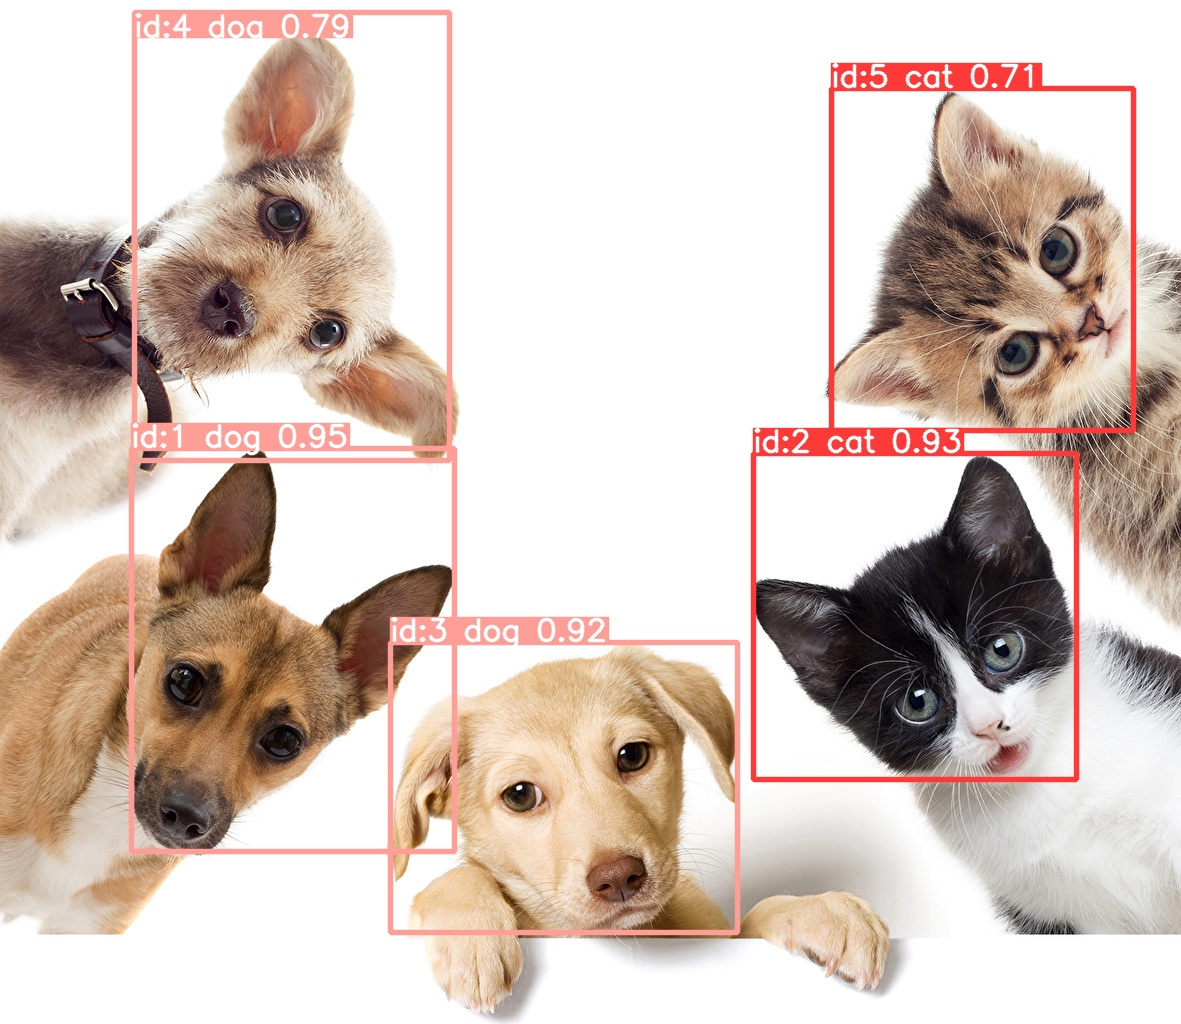
\includegraphics{predicts/predict 1.jpg} &
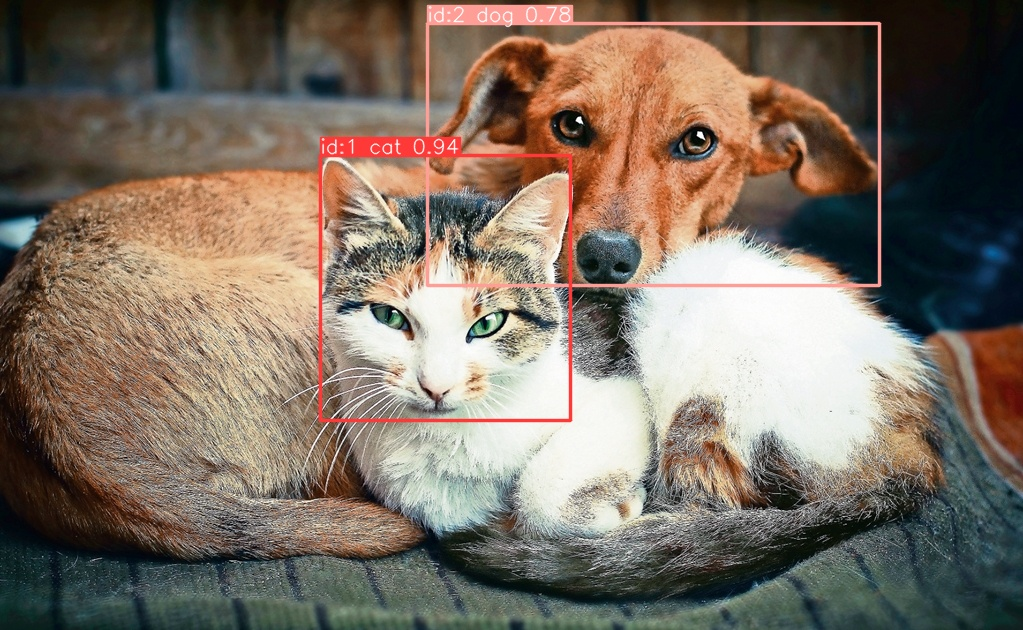
\includegraphics{predicts/predict 2.jpg} &
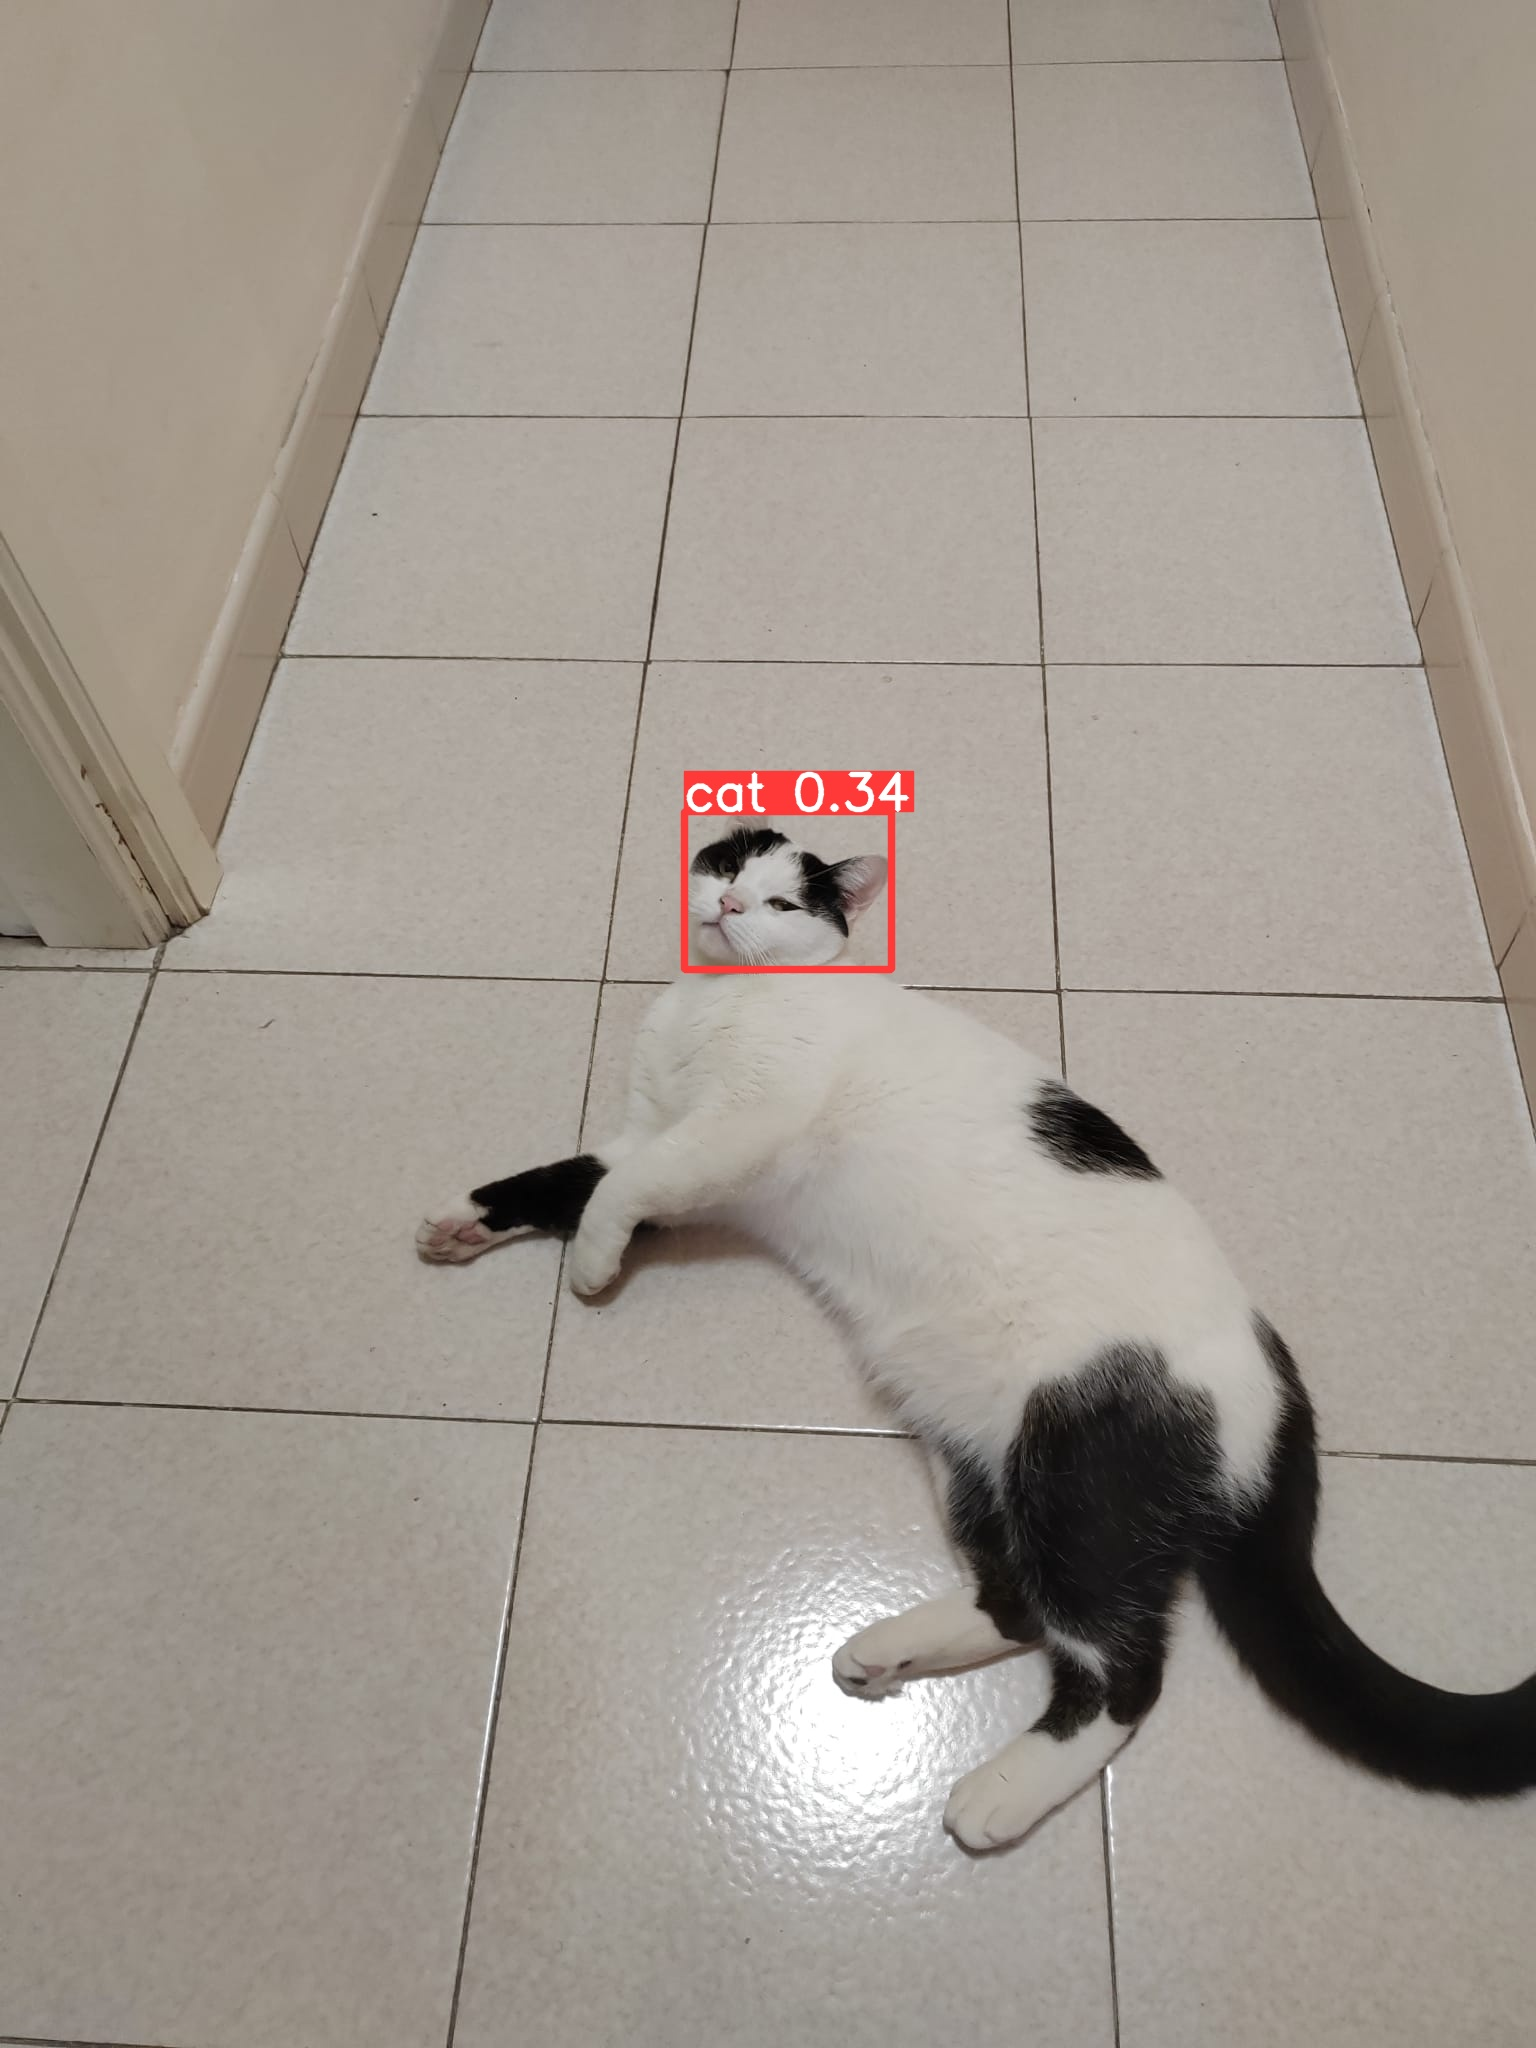
\includegraphics{predicts/predict 3.jpg} \\
\end{longtable}

    \subsection{Predicción con webcam}\label{predicciuxf3n-con-webcam}

    \begin{tcolorbox}[breakable, size=fbox, boxrule=1pt, pad at break*=1mm,colback=white, colframe=black]
\prompt{In}{incolor}{4}{\boxspacing}
\begin{Verbatim}[commandchars=\\\{\}]
\PY{k+kn}{from} \PY{n+nn}{ultralytics} \PY{k+kn}{import} \PY{n}{YOLO}

\PY{c+c1}{\PYZsh{} Cargar el modelo YOLO preentrenado}
\PY{n}{model} \PY{o}{=} \PY{n}{YOLO}\PY{p}{(}\PY{l+s+s2}{\PYZdq{}}\PY{l+s+s2}{results/weights/best.pt}\PY{l+s+s2}{\PYZdq{}}\PY{p}{)}
\PY{c+c1}{\PYZsh{} Realizar la predicción en una imagen}
\PY{n}{results} \PY{o}{=} \PY{n}{model}\PY{o}{.}\PY{n}{track}\PY{p}{(}\PY{n}{source}\PY{o}{=}\PY{l+m+mi}{1}\PY{p}{,} \PY{n}{conf}\PY{o}{=}\PY{l+m+mf}{0.3}\PY{p}{,}
\PY{n}{iou}\PY{o}{=}\PY{l+m+mf}{0.5}\PY{p}{,} \PY{n}{stream}\PY{o}{=}\PY{k+kc}{True}\PY{p}{,} \PY{n}{show}\PY{o}{=}\PY{k+kc}{True}\PY{p}{)} 

\PY{c+c1}{\PYZsh{} Process results list}
\PY{k}{for} \PY{n}{result} \PY{o+ow}{in} \PY{n}{results}\PY{p}{:}
    \PY{n}{boxes} \PY{o}{=} \PY{n}{result}\PY{o}{.}\PY{n}{boxes}
    \PY{k}{for} \PY{n}{box} \PY{o+ow}{in} \PY{n}{boxes}\PY{p}{:}
        \PY{n+nb}{print}\PY{p}{(}\PY{l+s+s2}{\PYZdq{}}\PY{l+s+s2}{Box:}\PY{l+s+s2}{\PYZdq{}}\PY{p}{,} \PY{n}{box}\PY{p}{)} 
\end{Verbatim}
\end{tcolorbox}

\begin{tcolorbox}[breakable, size=fbox, boxrule=1pt, pad at break*=1mm,colback=cellbackground, colframe=cellborder]
    \prompt{Out}{outcolor}{4}{\boxspacing}
    \begin{Verbatim}[commandchars=\\\{\}]

1/1: 1{\ldots} Success  (inf frames of shape 640x480 at 30.00 FPS)

0: 480x640 (no detections), 93.4ms
0: 480x640 (no detections), 87.1ms
0: 480x640 (no detections), 88.5ms
0: 480x640 (no detections), 89.0ms
0: 480x640 1 dog, 81.8ms
Box: ultralytics.engine.results.Boxes object with attributes:

cls: tensor([1.])
conf: tensor([0.5558])
data: tensor([[242.2409, 172.9478, 481.7175, 478.2041,   0.5558,   1.0000]])
id: None
is\_track: False
orig\_shape: (480, 640)
shape: torch.Size([1, 6])
xywh: tensor([[361.9792, 325.5760, 239.4766, 305.2562]])
xywhn: tensor([[0.5656, 0.6783, 0.3742, 0.6360]])
xyxy: tensor([[242.2409, 172.9478, 481.7175, 478.2041]])
xyxyn: tensor([[0.3785, 0.3603, 0.7527, 0.9963]])
0: 480x640 (no detections), 83.8ms
0: 480x640 (no detections), 93.2ms
0: 480x640 (no detections), 91.4ms
0: 480x640 (no detections), 81.3ms
0: 480x640 (no detections), 81.3ms
0: 480x640 (no detections), 78.7ms
0: 480x640 (no detections), 84.3ms
0: 480x640 (no detections), 80.8ms
0: 480x640 (no detections), 86.5ms
0: 480x640 1 dog, 83.8ms
Box: ultralytics.engine.results.Boxes object with attributes:
    \end{Verbatim}
\end{tcolorbox}

\newpage

\paragraph{Resultados}\label{resultados-webcam}
    \begin{longtable}[]{@{}
  >{\centering\arraybackslash}p{(\columnwidth - 4\tabcolsep) * \real{0.3333}}
  >{\centering\arraybackslash}p{(\columnwidth - 4\tabcolsep) * \real{0.3333}}
  >{\centering\arraybackslash}p{(\columnwidth - 4\tabcolsep) * \real{0.3333}}@{}}
\toprule\noalign{}
\begin{minipage}[b]{\linewidth}\centering
Imagen 1
\end{minipage} & \begin{minipage}[b]{\linewidth}\centering
Imagen 2
\end{minipage} & \begin{minipage}[b]{\linewidth}\centering
Imagen 3
\end{minipage} \\
\midrule\noalign{}
\endhead
\bottomrule\noalign{}
\endlastfoot
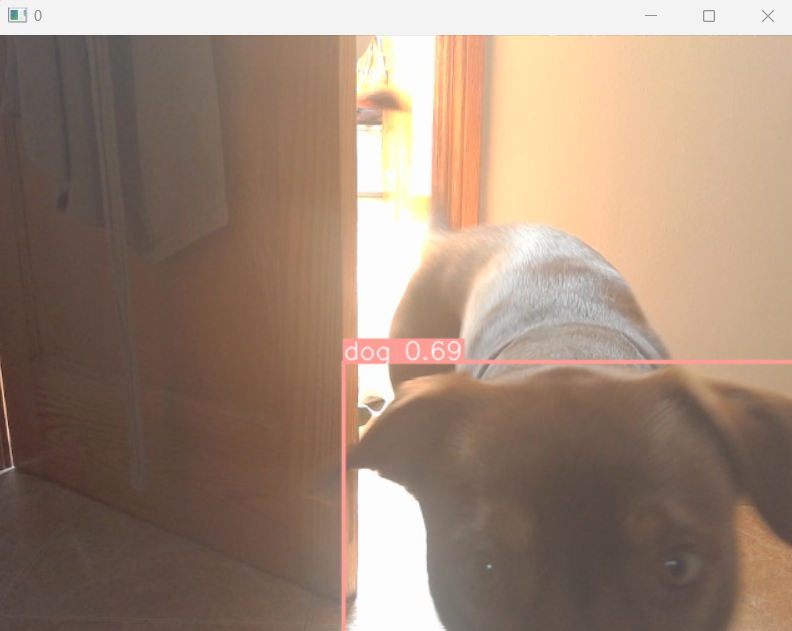
\includegraphics{predicts/Captura de pantalla 2024-05-08 142545.png} &
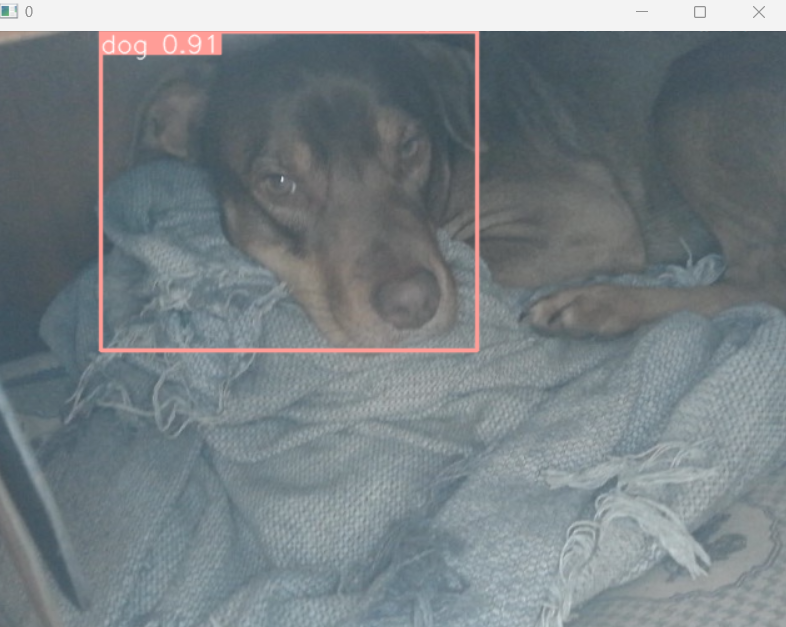
\includegraphics{predicts/Captura de pantalla 2024-05-08 142656.png} &
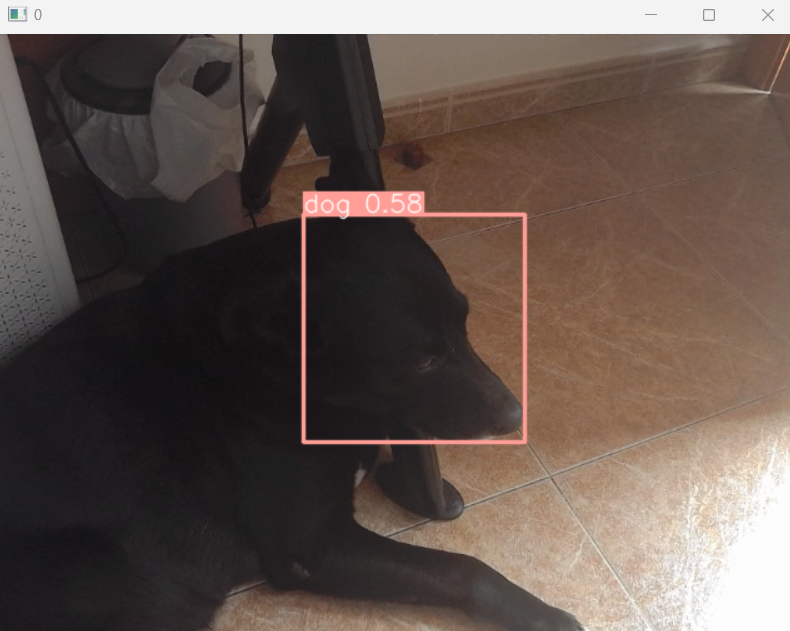
\includegraphics{predicts/Captura de pantalla 2024-05-08 142922.png} \\
\end{longtable}


    % Add a bibliography block to the postdoc
    
    
    
\end{document}
